% Options for packages loaded elsewhere
\PassOptionsToPackage{unicode}{hyperref}
\PassOptionsToPackage{hyphens}{url}
\PassOptionsToPackage{dvipsnames,svgnames,x11names}{xcolor}
%
\documentclass[
  11pt,
]{krantz}
\usepackage{amsmath,amssymb}
\usepackage{lmodern}
\usepackage{iftex}
\ifPDFTeX
  \usepackage[T1]{fontenc}
  \usepackage[utf8]{inputenc}
  \usepackage{textcomp} % provide euro and other symbols
\else % if luatex or xetex
  \usepackage{unicode-math}
  \defaultfontfeatures{Scale=MatchLowercase}
  \defaultfontfeatures[\rmfamily]{Ligatures=TeX,Scale=1}
  \setmonofont[Scale=0.775]{MesloLGS NF}
\fi
% Use upquote if available, for straight quotes in verbatim environments
\IfFileExists{upquote.sty}{\usepackage{upquote}}{}
\IfFileExists{microtype.sty}{% use microtype if available
  \usepackage[]{microtype}
  \UseMicrotypeSet[protrusion]{basicmath} % disable protrusion for tt fonts
}{}
\makeatletter
\@ifundefined{KOMAClassName}{% if non-KOMA class
  \IfFileExists{parskip.sty}{%
    \usepackage{parskip}
  }{% else
    \setlength{\parindent}{0pt}
    \setlength{\parskip}{6pt plus 2pt minus 1pt}}
}{% if KOMA class
  \KOMAoptions{parskip=half}}
\makeatother
\usepackage{xcolor}
\IfFileExists{xurl.sty}{\usepackage{xurl}}{} % add URL line breaks if available
\IfFileExists{bookmark.sty}{\usepackage{bookmark}}{\usepackage{hyperref}}
\hypersetup{
  pdftitle={Data Science per psicologi},
  pdfauthor={Corrado Caudek},
  colorlinks=true,
  linkcolor={Maroon},
  filecolor={Maroon},
  citecolor={Blue},
  urlcolor={Blue},
  pdfcreator={LaTeX via pandoc}}
\urlstyle{same} % disable monospaced font for URLs
\usepackage{color}
\usepackage{fancyvrb}
\newcommand{\VerbBar}{|}
\newcommand{\VERB}{\Verb[commandchars=\\\{\}]}
\DefineVerbatimEnvironment{Highlighting}{Verbatim}{commandchars=\\\{\}}
% Add ',fontsize=\small' for more characters per line
\usepackage{framed}
\definecolor{shadecolor}{RGB}{248,248,248}
\newenvironment{Shaded}{\begin{snugshade}}{\end{snugshade}}
\newcommand{\AlertTok}[1]{\textcolor[rgb]{0.33,0.33,0.33}{#1}}
\newcommand{\AnnotationTok}[1]{\textcolor[rgb]{0.37,0.37,0.37}{\textbf{\textit{#1}}}}
\newcommand{\AttributeTok}[1]{\textcolor[rgb]{0.61,0.61,0.61}{#1}}
\newcommand{\BaseNTok}[1]{\textcolor[rgb]{0.06,0.06,0.06}{#1}}
\newcommand{\BuiltInTok}[1]{#1}
\newcommand{\CharTok}[1]{\textcolor[rgb]{0.5,0.5,0.5}{#1}}
\newcommand{\CommentTok}[1]{\textcolor[rgb]{0.37,0.37,0.37}{\textit{#1}}}
\newcommand{\CommentVarTok}[1]{\textcolor[rgb]{0.37,0.37,0.37}{\textbf{\textit{#1}}}}
\newcommand{\ConstantTok}[1]{\textcolor[rgb]{0,0,0}{#1}}
\newcommand{\ControlFlowTok}[1]{\textcolor[rgb]{0.27,0.27,0.27}{\textbf{#1}}}
\newcommand{\DataTypeTok}[1]{\textcolor[rgb]{0.27,0.27,0.27}{#1}}
\newcommand{\DecValTok}[1]{\textcolor[rgb]{0.06,0.06,0.06}{#1}}
\newcommand{\DocumentationTok}[1]{\textcolor[rgb]{0.37,0.37,0.37}{\textbf{\textit{#1}}}}
\newcommand{\ErrorTok}[1]{\textcolor[rgb]{0.14,0.14,0.14}{\textbf{#1}}}
\newcommand{\ExtensionTok}[1]{#1}
\newcommand{\FloatTok}[1]{\textcolor[rgb]{0.06,0.06,0.06}{#1}}
\newcommand{\FunctionTok}[1]{\textcolor[rgb]{0,0,0}{#1}}
\newcommand{\ImportTok}[1]{#1}
\newcommand{\InformationTok}[1]{\textcolor[rgb]{0.37,0.37,0.37}{\textbf{\textit{#1}}}}
\newcommand{\KeywordTok}[1]{\textcolor[rgb]{0.27,0.27,0.27}{\textbf{#1}}}
\newcommand{\NormalTok}[1]{#1}
\newcommand{\OperatorTok}[1]{\textcolor[rgb]{0.43,0.43,0.43}{\textbf{#1}}}
\newcommand{\OtherTok}[1]{\textcolor[rgb]{0.37,0.37,0.37}{#1}}
\newcommand{\PreprocessorTok}[1]{\textcolor[rgb]{0.37,0.37,0.37}{\textit{#1}}}
\newcommand{\RegionMarkerTok}[1]{#1}
\newcommand{\SpecialCharTok}[1]{\textcolor[rgb]{0,0,0}{#1}}
\newcommand{\SpecialStringTok}[1]{\textcolor[rgb]{0.5,0.5,0.5}{#1}}
\newcommand{\StringTok}[1]{\textcolor[rgb]{0.5,0.5,0.5}{#1}}
\newcommand{\VariableTok}[1]{\textcolor[rgb]{0,0,0}{#1}}
\newcommand{\VerbatimStringTok}[1]{\textcolor[rgb]{0.5,0.5,0.5}{#1}}
\newcommand{\WarningTok}[1]{\textcolor[rgb]{0.37,0.37,0.37}{\textbf{\textit{#1}}}}
\usepackage{longtable,booktabs,array}
\usepackage{calc} % for calculating minipage widths
% Correct order of tables after \paragraph or \subparagraph
\usepackage{etoolbox}
\makeatletter
\patchcmd\longtable{\par}{\if@noskipsec\mbox{}\fi\par}{}{}
\makeatother
% Allow footnotes in longtable head/foot
\IfFileExists{footnotehyper.sty}{\usepackage{footnotehyper}}{\usepackage{footnote}}
\makesavenoteenv{longtable}
\usepackage{graphicx}
\makeatletter
\def\maxwidth{\ifdim\Gin@nat@width>\linewidth\linewidth\else\Gin@nat@width\fi}
\def\maxheight{\ifdim\Gin@nat@height>\textheight\textheight\else\Gin@nat@height\fi}
\makeatother
% Scale images if necessary, so that they will not overflow the page
% margins by default, and it is still possible to overwrite the defaults
% using explicit options in \includegraphics[width, height, ...]{}
\setkeys{Gin}{width=\maxwidth,height=\maxheight,keepaspectratio}
% Set default figure placement to htbp
\makeatletter
\def\fps@figure{htbp}
\makeatother
\setlength{\emergencystretch}{3em} % prevent overfull lines
\providecommand{\tightlist}{%
  \setlength{\itemsep}{0pt}\setlength{\parskip}{0pt}}
\setcounter{secnumdepth}{5}
\usepackage{amsmath}
\usepackage{amssymb}
\usepackage{amsfonts}

\defaultfontfeatures{Scale=MatchLowercase}

\usepackage{booktabs}
\usepackage{longtable}
\usepackage[bf,singlelinecheck=off]{caption}

\usepackage{framed,color}
\definecolor{shadecolor}{RGB}{248,248,248}

\renewcommand{\textfraction}{0.05}
\renewcommand{\topfraction}{0.8}
\renewcommand{\bottomfraction}{0.8}
\renewcommand{\floatpagefraction}{0.75}

\renewenvironment{quote}{\begin{VF}}{\end{VF}}
\let\oldhref\href
\renewcommand{\href}[2]{#2\footnote{\url{#1}}}

\ifxetex
  \usepackage{letltxmacro}
  \setlength{\XeTeXLinkMargin}{1pt}
  \LetLtxMacro\SavedIncludeGraphics\includegraphics
  \def\includegraphics#1#{% #1 catches optional stuff (star/opt. arg.)
    \IncludeGraphicsAux{#1}%
  }%
  \newcommand*{\IncludeGraphicsAux}[2]{%
    \XeTeXLinkBox{%
      \SavedIncludeGraphics#1{#2}%
    }%
  }%
\fi

\makeatletter
\newenvironment{kframe}{%
\medskip{}
\setlength{\fboxsep}{.8em}
 \def\at@end@of@kframe{}%
 \ifinner\ifhmode%
  \def\at@end@of@kframe{\end{minipage}}%
  \begin{minipage}{\columnwidth}%
 \fi\fi%
 \def\FrameCommand##1{\hskip\@totalleftmargin \hskip-\fboxsep
 \colorbox{shadecolor}{##1}\hskip-\fboxsep
     % There is no \\@totalrightmargin, so:
     \hskip-\linewidth \hskip-\@totalleftmargin \hskip\columnwidth}%
 \MakeFramed {\advance\hsize-\width
   \@totalleftmargin\z@ \linewidth\hsize
   \@setminipage}}%
 {\par\unskip\endMakeFramed%
 \at@end@of@kframe}
\makeatother

\renewenvironment{Shaded}{\begin{kframe}}{\end{kframe}}

\usepackage{makeidx}
\makeindex

\urlstyle{tt}

\usepackage{amsthm}
\makeatletter
\def\thm@space@setup{%
  \thm@preskip=8pt plus 2pt minus 4pt
  \thm@postskip=\thm@preskip
}
\makeatother

\DeclareMathOperator{\V}{\mathbb{V}} % Define variance operator
\DeclareMathOperator{\Var}{\mathbb{V}} % Define variance operator
\DeclareMathOperator{\SD}{SD} % Define sd operator
\DeclareMathOperator{\Cov}{Cov} % Define covariance operator
\DeclareMathOperator{\Corr}{Corr} % Define correlation operator
\DeclareMathOperator{\Me}{Me} % Define mediane operator
\DeclareMathOperator{\Mo}{Mo} % Define mode operator

\DeclareMathOperator{\Bin}{Binomial} % Define binomial operator
\DeclareMathOperator{\Bernoulli}{Bernoulli} % Define Bernoulli operator
\DeclareMathOperator{\Ber}{\mathscr{B}} % Define Bernoulli operator
\DeclareMathOperator{\Poi}{Poisson} % Define Poisson operator
\DeclareMathOperator{\Uniform}{Uniform} % Define Uniform operator
\DeclareMathOperator{\Cauchy}{Cauchy} % Define Cauchy operator
\DeclareMathOperator{\B}{B} % beta function
% \mbox{B}(a, b) % beta function
% \mbox{Beta}(a, b) % beta distribution

\DeclareMathOperator{\elpd}{elpd} % Define elpd operator
\DeclareMathOperator{\lppd}{lppd} % Define lppd operator
\DeclareMathOperator{\LOO}{LOO} % Define LOO operator
\DeclareMathOperator{\argmin}{arg\,min} 
\DeclareMathOperator{\argmax}{arg\,max} 

\newcommand{\E}{\mathbb{E}} % Define expected value operator
\newcommand{\R}{\textsf{R}} % Define R programming language symbol
\newcommand{\Real}{\mathbb{R}} % Define real number operator
\newcommand{\Prob}{\mathscr{P}}
\newcommand{\indep}{\perp \!\!\! \perp}

\usepackage[
 labelfont=bf,
 font={small, it}
]{caption}
\usepackage{upquote} % print correct quotes in verbatim-environments
\usepackage{empheq}
\usepackage{xfrac}

\usepackage{polyglossia}
\setmainlanguage{italian}

\frontmatter
\ifLuaTeX
  \usepackage{selnolig}  % disable illegal ligatures
\fi
\usepackage[]{natbib}
\bibliographystyle{apalike}

\title{Data Science per psicologi}
\author{Corrado Caudek}
\date{2022-02-13}

\usepackage{amsthm}
\newtheorem{theorem}{Teorema}[chapter]
\newtheorem{lemma}{Lemma}[chapter]
\newtheorem{corollary}{Corollario}[chapter]
\newtheorem{proposition}{Proposizione}[chapter]
\newtheorem{conjecture}{Congettura}[chapter]
\theoremstyle{definition}
\newtheorem{definition}{Definizione}[chapter]
\theoremstyle{definition}
\newtheorem{example}{Esempio}[chapter]
\theoremstyle{definition}
\newtheorem{exercise}{Esercizio}[chapter]
\theoremstyle{definition}
\newtheorem{hypothesis}{Hypothesis}[chapter]
\theoremstyle{remark}
\newtheorem*{remark}{Osservazione}
\newtheorem*{solution}{Soluzione}
\begin{document}
\maketitle

\cleardoublepage\newpage\thispagestyle{empty}\null
% \cleardoublepage\newpage\thispagestyle{empty}\null
%\cleardoublepage\newpage
\thispagestyle{empty}
\begin{center}
\Large{Psicometria -- AA 2021/2022}

\vskip20pt

\includegraphics{images/confounding_variables.png}
\end{center}

\setlength{\abovedisplayskip}{-5pt}
\setlength{\abovedisplayshortskip}{-5pt}

{
\hypersetup{linkcolor=}
\setcounter{tocdepth}{2}
\tableofcontents
}
\listoffigures
\listoftables
\hypertarget{prefazione}{%
\chapter*{Prefazione}\label{prefazione}}


\emph{Data Science per psicologi} contiene il materiale delle lezioni dell'insegnamento di \emph{Psicometria B000286} (A.A. 2021/2022) rivolto agli studenti del primo anno del Corso di Laurea in Scienze e Tecniche Psicologiche dell'Università degli Studi di Firenze. \emph{Psicometria} si propone di fornire agli studenti un'introduzione all'analisi dei dati in psicologia. Le conoscenze/competenze che verranno sviluppate in questo insegnamento sono quelle della Data science, ovvero un insieme di conoscenze/competenze che si pongono all'intersezione tra statistica (ovvero, richiedono la capacità di comprendere teoremi statistici) e informatica (ovvero, richiedono la capacità di sapere utilizzare un software).

\hypertarget{la-psicologia-e-la-data-science}{%
\section*{La psicologia e la Data science}\label{la-psicologia-e-la-data-science}}


Sembra sensato spendere due parole su un tema che è importante per gli studenti: quello indicato dal titolo di questo Capitolo. È ovvio che agli studenti di psicologia la statistica non piace. Se piacesse, forse studierebbero Data science e non psicologia; ma non lo fanno. Di conseguenza, gli studenti di psicologia si chiedono: ``perché dobbiamo perdere tanto tempo a studiare queste cose quando in realtà quello che ci interessa è tutt'altro?'' Questa è una bella domanda.

C'è una ragione molto semplice che dovrebbe farci capire perché la Data science è così importante per la psicologia. Infatti, a ben pensarci, la psicologia è una disciplina intrinsecamente statistica, se per statistica intendiamo quella disciplina che studia la variazione delle caratteristiche degli individui nella popolazione. La psicologia studia \emph{gli individui} ed è proprio la variabilità inter- e intra-individuale ciò che vogliamo descrivere e, in certi casi, predire. In questo senso, la psicologia è molto diversa dall'ingegneria, per esempio. Le proprietà di un determinato ponte sotto certe condizioni, ad esempio, sono molto simili a quelle di un altro ponte, sotto le medesime condizioni. Quindi, per un ingegnere la statistica è poco importante: le proprietà dei materiali sono unicamente dipendenti dalla loro composizione e restano costanti. Ma lo stesso non può dirsi degli individui: ogni individuo è unico e cambia nel tempo. E le variazioni tra gli individui, e di un individuo nel tempo, sono l'oggetto di studio proprio della psicologia: è dunque chiaro che i problemi che la psicologia si pone sono molto diversi da quelli affrontati, per esempio, dagli ingegneri. Questa è la ragione per cui abbiamo tanto bisogno della Data science in psicologia: perché la Data science ci consente di descrivere la variazione e il cambiamento. E queste sono appunto le caratteristiche di base dei fenomeni psicologici.

Sono sicuro che, leggendo queste righe, a molti studenti sarà venuta in mente la seguente domanda: perché non chiediamo a qualche esperto di fare il ``lavoro sporco'' (ovvero le analisi statistiche) per noi, mentre noi (gli psicologi) ci occupiamo solo di ciò che ci interessa, ovvero dei problemi psicologici slegati dai dettagli ``tecnici'' della Data science? La risposta a questa domanda è che non è possibile progettare uno studio psicologico sensato senza avere almeno una comprensione rudimentale della Data science. Le tematiche della Data science non possono essere ignorate né dai ricercatori in psicologia né da coloro che svolgono la professione di psicologo al di fuori dell'Università. Infatti, anche i professionisti al di fuori dall'università non possono fare a meno di leggere la letteratura psicologica più recente: il continuo aggiornamento delle conoscenze è infatti richiesto dalla deontologia della professione. Ma per potere fare questo è necessario conoscere un bel po' di Data science! Basta aprire a caso una rivista specialistica di psicologia per rendersi conto di quanto ciò sia vero: gli articoli che riportano i risultati delle ricerche psicologiche sono zeppi di analisi statistiche e di modelli formali. E la comprensione della letteratura psicologica rappresenta un requisito minimo nel bagaglio professionale dello psicologo.

Le considerazioni precedenti cercano di chiarire il seguente punto: la Data science non è qualcosa da studiare a malincuore, in un singolo insegnamento universitario, per poi poterla tranquillamente dimenticare. Nel bene e nel male, gli psicologi usano gli strumenti della Data science in tantissimi ambiti della loro attività professionale: in particolare quando costruiscono, somministrano e interpretano i test psicometrici. È dunque chiaro che possedere delle solide basi di Data science è un tassello imprescindibile del bagaglio professionale dello psicologo. In questo insegnamento verrano trattati i temi base della Data science e verrà adottato un punto di vista bayesiano, che corrisponde all'approccio più recente e sempre più diffuso in psicologia.

\hypertarget{come-studiare}{%
\section*{Come studiare}\label{come-studiare}}


Il giusto metodo di studio per prepararsi all'esame di Psicometria è quello di seguire attivamente le lezioni, assimilare i concetti via via che essi vengono presentati e verificare in autonomia le procedure presentate a lezione. Incoraggio gli studenti a farmi domande per chiarire ciò che non è stato capito appieno. Incoraggio gli studenti a utilizzare i forum attivi su Moodle e, soprattutto, a svolgere gli esercizi proposti su Moodle. I problemi forniti su Moodle rappresentano il livello di difficoltà richiesto per superare l'esame e consentono allo studente di comprendere se le competenze sviluppate fino a quel punto sono sufficienti rispetto alle richieste dell'esame.

La prima fase dello studio, che è sicuramente individuale, è quella in cui è necessario acquisire le conoscenze teoriche relative ai problemi che saranno presentati all'esame. La seconda fase di studio, che può essere facilitata da scambi con altri e da incontri di gruppo, porta ad acquisire la capacità di applicare le conoscenze: è necessario capire come usare un software (\(\textsf{R}\)) per applicare i concetti statistici alla specifica situazione del problema che si vuole risolvere. Le due fasi non sono però separate: il saper fare molto spesso ci aiuta a capire meglio.

\hypertarget{sviluppare-un-metodo-di-studio-efficace}{%
\section*{Sviluppare un metodo di studio efficace}\label{sviluppare-un-metodo-di-studio-efficace}}


Avendo insegnato molte volte in passato un corso introduttivo di analisi dei dati ho notato nel corso degli anni che gli studenti con l'atteggiamento mentale che descriverò qui sotto generalmente ottengono ottimi risultati. Alcuni studenti sviluppano naturalmente questo approccio allo studio, ma altri hanno bisogno di fare uno sforzo per maturarlo. Fornisco qui sotto una breve descrizione del ``metodo di studio'' che, nella mia esperienza, è il più efficace per affrontare le richieste di questo insegnamento.

\begin{itemize}
\tightlist
\item
  Dedicate un tempo sufficiente al materiale di base, apparentemente facile; assicuratevi di averlo capito bene. Cercate le lacune nella vostra comprensione. Leggere presentazioni diverse dello stesso materiale (in libri o articoli diversi) può fornire nuove intuizioni.
\item
  Gli errori che facciamo sono i nostri migliori maestri. Istintivamente cerchiamo di dimenticare subito i nostri errori. Ma il miglior modo di imparare è apprendere dagli errori che commettiamo. In questo senso, una soluzione corretta è meno utile di una soluzione sbagliata. Quando commettiamo un errore questo ci fornisce un'informazione importante: ci fa capire qual è il materiale di studio sul quale dobbiamo ritornare e che dobbiamo capire meglio.
\item
  C'è ovviamente un aspetto ``psicologico'' nello studio. Quando un esercizio o problema ci sembra incomprensibile, la cosa migliore da fare è dire: ``mi arrendo'', ``non ho idea di cosa fare!''. Questo ci rilassa: ci siamo già arresi, quindi non abbiamo niente da perdere, non dobbiamo più preoccuparci. Ma non dobbiamo fermarci qui. Le cose ``migliori'' che faccio (se ci sono) le faccio quando non ho voglia di lavorare. Alle volte, quando c'è qualcosa che non so fare e non ho idea di come affontare, mi dico: ``oggi non ho proprio voglia di fare fatica'', non ho voglia di mettermi nello stato mentale per cui ``in 10 minuti devo risolvere il problema perché dopo devo fare altre cose''. Però ho voglia di \emph{divertirmi} con quel problema e allora mi dedico a qualche aspetto ``marginale'' del problema, che so come affrontare, oppure considero l'aspetto più difficile del problema, quello che non so come risolvere, ma invece di cercare di risolverlo, guardo come altre persone hanno affrontato problemi simili, opppure lo stesso problema in un altro contesto. Non mi pongo l'obiettivo ``risolvi il problema in 10 minuti'', ma invece quello di farmi un'idea ``generale'' del problema, o quello di capire un caso più specifico e più semplice del problema. Senza nessuna pressione. Infatti, in quel momento ho deciso di non lavorare (ovvero, di non fare fatica). Va benissimo se ``parto per la tangente'', ovvero se mi metto a leggere del materiale che sembra avere poco a che fare con il problema centrale (le nostre intuizioni e la nostra curiosità solitamente ci indirizzano sulla strada giusta). Quando faccio così, molto spesso trovo la soluzione del problema che mi ero posto e, paradossalmente, la trovo in un tempo minore di quello che, in precedenza, avevo dedicato a ``lavorare'' al problema. Allora perché non faccio sempre così? C'è ovviamente l'aspetto dei ``10 minuti'' che non è sempre facile da dimenticare. Sotto pressione, possiamo solo agire in maniera automatica, ovvero possiamo solo applicare qualcosa che già sappiamo fare. Ma se dobbiamo imparare qualcosa di nuovo, la pressione è un impedimento.
\item
  È utile farsi da soli delle domande sugli argomenti trattati, senza limitarsi a cercare di risolvere gli esercizi che vengono assegnati. Quando studio qualcosa mi viene in mente: ``se questo è vero, allora deve succedere quest'altra cosa''. Allora verifico se questo è vero, di solito con una simulazione. Se i risultati della simulazione sono quelli che mi aspetto, allora vuol dire che ho capito. Se i risultati sono diversi da quelli che mi aspettavo, allora mi rendo conto di non avere capito e ritorno indietro a studiare con più attenzione la teoria che pensavo di avere capito -- e ovviamente mi rendo conto che c'era un aspetto che avevo frainteso. Questo tipo di verifica è qualcosa che dobbiamo fare da soli, in prima persona: nessun altro può fare questo al posto nostro.
\item
  Non aspettatevi di capire tutto la prima volta che incontrate un argomento nuovo.\footnote{Ricordatevi inoltre che gli individui tendono a sottostimare la propria capacità di apprendere \citep{horn2021underestimating}.} È utile farsi una nota mentalmente delle lacune nella vostra comprensione e tornare su di esse in seguito per carcare di colmarle. L'atteggiamento naturale, quando non capiamo i dettagli di qualcosa, è quello di pensare: ``non importa, ho capito in maniera approssimativa questo punto, non devo preoccuparmi del resto''. Ma in realtà non è vero: se la nostra comprensione è superficiale, quando il problema verrà presentato in una nuova forma, non riusciremo a risolverlo. Per cui i dubbi che ci vengono quando studiamo qualcosa sono il nostro alleato più prezioso: ci dicono esattamente quali sono gli aspetti che dobbiamo approfondire per potere migliorare la nostra preparazione.
\item
  È utile sviluppare una visione d'insieme degli argomenti trattati, capire l'obiettivo generale che si vuole raggiungere e avere chiaro il contributo che i vari pezzi di informazione forniscono al raggiungimento di tale obiettivo. Questa organizzazione mentale del materiale di studio facilita la comprensione. È estremamente utile creare degli schemi di ciò che si sta studiando. Non aspettate che sia io a fornirvi un riepilogo di ciò che dovete imparare: sviluppate da soli tali schemi e tali riassunti.
\item
  Tutti noi dobbiamo imparare l'arte di trovare le informazioni, non solo nel caso di questo insegnamento. Quando vi trovate di fronte a qualcosa che non capite, o ottenete un oscuro messaggio di errore da un software, ricordatevi: ``Google is your friend''!
\end{itemize}

\begin{flushright}
Corrado Caudek\\
Marzo 2022 \end{flushright}

\mainmatter

\hypertarget{part-inferenza-bayesiana}{%
\part{Inferenza bayesiana}\label{part-inferenza-bayesiana}}

\hypertarget{ch:intro-bayes-inference}{%
\chapter{Flusso di lavoro bayesiano}\label{ch:intro-bayes-inference}}

La moderna statistica bayesiana viene per lo più eseguita utilizzando un linguaggio di programmazione probabilistico implementato su computer. Ciò ha cambiato radicalmente il modo in cui venivano eseguite le statistiche bayesiane anche fin pochi decenni fa. La complessità dei modelli che possiamo costruire è aumentata e la barriera delle competenze matematiche e computazionali che sono richieste è diminuita. Inoltre, il processo di modellazione iterativa è diventato, sotto molti aspetti, molto più facile da eseguire. Anche se formulare modelli statistici complessi è diventato più facile che mai, la statistica è un campo pieno di sottigliezze che non scompaiono magicamente utilizzando potenti metodi computazionali. Pertanto, avere una buona preparazione sugli aspetti teorici, specialmente quelli rilevanti nella pratica, è estremamente utile per applicare efficacemente i metodi statistici.

\hypertarget{modellizzazione-bayesiana}{%
\section{Modellizzazione bayesiana}\label{modellizzazione-bayesiana}}

L'analisi bayesiana corrisponde alla costruzione di un modello statistico che si può rappresentare con una quaterna

\begin{equation}
(\mathcal{Y}, p(y \mid \theta), p(\theta), \theta \in \Theta),
\end{equation}

dove \(\mathcal{Y}\) è l'insieme di tutti i possibili risultati ottenuti dall'esperimento casuale e \(p(y \mid \theta)\) è una famiglia di leggi di probabilità, indicizzata dal parametro \(\theta \in \Theta\), che descrive l'incertezza sull'esito dell'esperimento. Secondo l'approccio bayesiano, il parametro incognito \(\theta\) è considerato una variabile casuale che segue la legge di probabilità \(p(\theta)\). L'incertezza su \(\theta\) è la sintesi delle opinioni e delle informazioni che si hanno sul parametro prima di avere osservato il risultato dell'esperimento e prende il nome di \emph{distribuzione a priori}. La costruzione del modello statistico passa attraverso la scelta di una densità \(p(y \mid \theta)\) che rappresenta, in senso probabilistico, il fenomeno d'interesse, e attraverso la scelta di una distribuzione a priori \(p(\theta)\). Le informazioni che si hanno a priori sul parametro di interesse \(\theta\), contenute in \(p(\theta)\), vengono aggiornate attraverso quelle provenienti dal campione osservato \(y = (y_1, \dots, y_n)\) contenute nella funzione \(p(y \mid \theta)\), che, osservata come funzione di \(\theta\) per \(y\), prende il nome di \emph{funzione di verosimiglianza}. L'aggiornamento delle informazioni avviene attraverso la formula di Bayes

\begin{equation}
p(\theta \mid y) = \frac{p(y \mid \theta) p(\theta)}{\int_{\Theta}p(y \mid \theta) p(\theta) \,\operatorname {d}\!\theta} \quad \theta \in \Theta,
 \label{eq:bayes-intro}
\end{equation}

in cui \(p(\theta \mid y)\) prende il nome di \emph{distribuzione a posteriori}.

Il denominatore del Teorema di Bayes \eqref{eq:bayes-intro}, che costituisce la costante di normalizzazione, è la densità marginale dei dati (o verosimiglianza marginale). In ambito bayesiano la distribuzione a posteriori viene utilizzata per calcolare le principali quantità di interesse dell'inferenza, ad esempio la media a posteriori di \(\theta\).

Possiamo descrivere la modellazione bayesiana distinguendo tre passaggi \citep{martin2022bayesian}.

\begin{enumerate}
\def\labelenumi{\arabic{enumi}.}
\tightlist
\item
  Dati alcuni dati e alcune ipotesi su come questi dati potrebbero essere stati generati, progettiamo un modello combinando e trasformando variabili casuali.
\item
  Usiamo il teorema di Bayes per condizionare i nostri modelli ai dati disponibili. Chiamiamo questo processo ``inferenza'' e come risultato otteniamo una distribuzione a posteriori.
\item
  Critichiamo il modello verificando se il modello abbia senso utilizzando criteri diversi, inclusi i dati e la nostra conoscenza del dominio. Poiché generalmente siamo incerti sui modelli, a volte confrontiamo modelli diversi.
\end{enumerate}

Questi tre passaggi vengono eseguiti in modo iterativo e danno luogo a quello che è chiamato ``flusso di lavoro bayesiano'' (\emph{bayesian workflow}).

\hypertarget{notazione}{%
\subsection{Notazione}\label{notazione}}

Per fissare la notazione, nel seguito \(y\) rappresenterà i dati e \(\theta\) rappresenterà i parametri incogniti di un modello statistico. Sia \(y\) che \(\theta\) vengono concepiti come variabili casuali. Con \(x\) vengono invece denotate le quantità note, come ad esempio i predittori del modello lineare. Per rappresentare in un modo conciso i modelli probabilistici viene usata una notazione particolare. Ad esempio, invece di scrivere \(p(\theta) = \mbox{Beta}(1, 1)\) scriviamo \(\theta \sim \mbox{Beta}(1, 1)\). Il simbolo ``\(\sim\)'' viene spesso letto ``è distribuito come''. Possiamo anche pensare che significhi che \(\theta\) costituisce un campione casuale estratto dalla distribuzione Beta(1, 1). Allo stesso modo, ad esempio, la verosimiglianza del modello binomiale può essere scritta come \(y \sim \text{Bin}(n, \theta)\).

\hypertarget{distribuzioni-a-priori}{%
\section{Distribuzioni a priori}\label{distribuzioni-a-priori}}

Quando adottiamo un approccio bayesiano, i parametri della distribuzione di riferimento non venono considerati come delle costanti incognite ma bensì vengono trattati come variabili casuali; di conseguenza, i parametri assumono una particolare distribuzione che nelle statistica bayesiana viene definita ``a priori''. I parametri (o il parametro), che possiamo indicare con \(\theta\), possono assumere delle distribuzioni a priori differenti: a seconda delle informazioni disponibili bisogna selezionare una distribuzione di \(\theta\) in modo tale che venga assegnata una probabilità maggiore a quei valori che si ritengono più plausibili per \(\theta\). Idealmente, le credenze a priori che portano alla specificazione di una distribuzione a priori dovrebbero essere supportate da una qualche motivazione, come ad esempio i risultati di ricerche precedenti.

\hypertarget{tipologie-di-distribuzioni-a-priori}{%
\subsection{Tipologie di distribuzioni a priori}\label{tipologie-di-distribuzioni-a-priori}}

Possiamo distinguere tra diverse distribuzioni a priori in base a quanto fortemente impegnano il ricercatore a ritenere come plausibile un particolare intervallo di valori dei parametri. Il caso più estremo è quello che rivela una totale assenza di conoscenze a priori, il che conduce alle \emph{distribuzioni a priori non informative}, ovvero quelle che assegnano lo stesso livello di credibilità a tutti i valori dei parametri. Le distribuzioni a priori informative, d'altra parte, possono essere \emph{debolmente informative} o \emph{fortemente informative}, a seconda della forza della credenza che esprimono. Il caso più estremo di credenza a priori è quello che riassume il punto di vista del ricercatore nei termini di un \emph{unico valore} del parametro, il che assegna tutta la probabilità (massa o densità) ad di un singolo valore del parametro. Poiché questa non è più una distribuzione di probabilità, sebbene ne soddisfi la definizione, in questo caso si parla di una \emph{distribuzione a priori degenerata}. La figura seguente motra alcuni esempi di distribuzioni a priori per il modello Binomiale:

\begin{itemize}
\tightlist
\item
  distribuzione \emph{non informativa}: \(\theta_c \sim \mbox{Beta}(1,1)\);
\item
  distribuzione \emph{debolmente informativa}: \(\theta_c \sim \mbox{Beta}(5,2)\);
\item
  distribuzione \emph{fortemente informativa}: \(\theta_c \sim \mbox{Beta}(50,20)\);
\item
  \emph{valore puntuale}: \(\theta_c \sim \mbox{Beta}(\alpha, \beta)\) con \(\alpha, \beta \rightarrow \infty\) e \(\frac{\alpha}{\beta} = \frac{5}{2}\).
\end{itemize}

\begin{figure}[h]

{\centering \includegraphics{ds4psy_files/figure-latex/unnamed-chunk-3-1} 

}

\caption{Esempi di distribuzioni a priori per il parametro $\theta_c$ nel Modello Binomiale.}\label{fig:unnamed-chunk-3}
\end{figure}

\hypertarget{selezione-della-distribuzione-a-priori}{%
\subsection{Selezione della distribuzione a priori}\label{selezione-della-distribuzione-a-priori}}

La selezione delle distribuzioni a priori è stata spesso vista come una delle scelte più importanti che un ricercatore fa quando implementa un modello bayesiano in quanto può avere un impatto sostanziale sui risultati finali. La soggettività delle distribuzioni a priori è evidenziata dai critici come un potenziale svantaggio dei metodi bayesiani. A questa critica, \citet{vandeSchoot2021modelling} rispondono dicendo che, al di là della scelta delle distribuzioni a priori, ci sono molti elementi del processo di inferenza statistica che sono soggettivi, ovvero la scelta del modello statistico e le ipotesi sulla distribuzione degli errori. In secondo luogo, \citet{vandeSchoot2021modelling} notano come le distribuzioni a priori svolgono due importanti ruoli statistici: quello della ``regolarizzazione della stima'', ovvero, il processo che porta ad indebolire l'influenza indebita di osservazioni estreme, e quello del miglioramento dell'efficienza della stima, ovvero, la facilitazione dei processi di calcolo numerico di stima della distribuzione a posteriori. L'effetto della distribuzione a priori sulla distribuzione a posteriori verrà discusso in dettaglio nel Capitolo \ref{chapter-balance}.

\hypertarget{unapplicazione-empirica}{%
\subsection{Un'applicazione empirica}\label{unapplicazione-empirica}}

Per introdurre la modelizzazione bayesiana useremo qui i dati riportati da \citet{zetschefuture2019} (si veda l'appendice \ref{appendix:future-exp}). Tali dati corrispondono a 23 ``successi'' in 30 prove e possono dunque essere considerati la manifestazione di una variabile casuale Bernoulliana.

Se non abbiamo alcuna informazione a priori su \(\theta\) (ovvero, la probabilità che l'aspettativa dell'umore futuro del partecipante sia distorta negativamente), potremmo pensare di usare una distribuzione a priori uniforme, ovvero una Beta di parametri \(\alpha=1\) e \(\beta=1\). Una tale scelta, tuttavia, è sconsigliata in quanto è più vantaggioso usare una distribuzione debolmente informativa, come ad esempio \(\mbox{Beta}(2, 2)\), che ha come scopo la regolarizzazione, cioè quello di mantenere le inferenze in un intervallo ragionevole. Qui useremo una \(\mbox{Beta}(2, 10)\).

\[
p(\theta) = \frac{\Gamma(12)}{\Gamma(2)\Gamma(10)}\theta^{2-1} (1-\theta)^{10-1}.
\]

\begin{Shaded}
\begin{Highlighting}[]
\NormalTok{bayesrules}\SpecialCharTok{::}\FunctionTok{plot\_beta}\NormalTok{(}\AttributeTok{alpha =} \DecValTok{2}\NormalTok{, }\AttributeTok{beta =} \DecValTok{10}\NormalTok{, }\AttributeTok{mean =} \ConstantTok{TRUE}\NormalTok{, }\AttributeTok{mode =} \ConstantTok{TRUE}\NormalTok{)}
\end{Highlighting}
\end{Shaded}

\begin{center}\includegraphics{ds4psy_files/figure-latex/unnamed-chunk-4-1} \end{center}

La \(\mbox{Beta}(2, 10)\) esprime la credenza che \(\theta\) assume valori \(< 0.5\), con il valore più plausibile pari a circa 0.1. Questo è assolutamente implausibile per il caso dell'esempio in discussione: la \(\mbox{Beta}(2, 10)\) verrà usata solo per scopi didattici, ovvero, per esplorare le conseguenze di tale scelta sulla distribuzione a posteriori.

\hypertarget{la-funzione-di-verosimiglianza}{%
\section{La funzione di verosimiglianza}\label{la-funzione-di-verosimiglianza}}

Iniziamo con una definizione.

\begin{definition}
La \emph{funzione di verosimiglianza} \(\mathcal{L}(\theta \mid y) = f(y \mid \theta), \theta \in \Theta,\) è la funzione di massa o di densità di probabilità dei dati \(y\) vista come una funzione del parametro sconosciuto (o dei parametri sconosciuti) \(\theta\).
\end{definition}

Detto in altre parole, le funzioni di verosimiglianza e di (massa o densità di) probabilità sono formalmente identiche, ma è completamente diversa la loro interpretazione. Nel caso della funzione di massa o di densità di probabilità la distribuzione del vettore casuale delle osservazioni campionarie \(y\) dipende dai valori assunti dal parametro (o dai parametri) \(\theta\); nel caso della la funzione di verosimiglianza la credibilità assegnata a ciascun possibile valore \(\theta\) viene determinata avendo acquisita l'informazione campionaria \(y\) che rappresenta l'elemento condizionante. In altri termini, la funzione di verosimiglianza descrive in termini relativi il sostegno empirico che \(\theta \in \Theta\) riceve da \(y\). Infatti, la funzione di verosimiglianza assume forme diverse al variare di \(y\). Possiamo dunque pensare alla funzione di verosimiglianza come alla risposta alla seguente domanda: avendo osservato i dati \(y\), quanto risultano (relativamente) credibili i diversi valori del parametro \(\theta\)? In termini più formali possiamo dire: sulla base dei dati, \(\theta_1 \in \Theta\) risulta più credibile di \(\theta_2 \in \Theta\) quale indice del modello probabilistico generatore dei dati se \(\mathcal{L}(\theta_1) > \mathcal{L}(\theta_1)\).

Notiamo un punto importante: la funzione \(\mathcal{L}(\theta \mid y)\) non è una funzione di densità. Infatti, essa non racchiude un'area unitaria.

\hypertarget{notazione-1}{%
\subsection{Notazione}\label{notazione-1}}

Seguendo una pratica comune, in questa dispensa spesso useremo la notazione \(p(\cdot)\) per rappresentare due quantità differenti, ovvero la funzione di verosimiglianza e la distribuzione a priori. Questo piccolo abuso di notazione riflette il seguente punto di vista: anche se la verosimiglianza non è una funzione di densità di probabilità, noi non vogliamo stressare questo aspetto, ma vogliamo piuttosto pensare alla verosimiglianza e alla distribuzione a priori come a due elementi che sono egualmente necessari per calcolare la distribuzione a posteriori. In altri termini, per così dire, questa notazione assegna lo stesso status epistemologico alle due diverse quantità che si trovano al numeratore della regola di Bayes.

\hypertarget{la-log-verosimiglianza}{%
\subsection{La log-verosimiglianza}\label{la-log-verosimiglianza}}

Dal punto di vista pratico risulta più conveniente utilizzare, al posto della funzione di verosimiglianza, il suo logaritmo naturale, ovvero la funzione di log-verosimiglianza:

\begin{equation}
\ell(\theta) = \log \mathcal{L}(\theta).
\end{equation}

Poiché il logaritmo è una funzione strettamente crescente (usualmente si considera il logaritmo naturale), allora \(\mathcal{L}(\theta)\) e \(\ell(\theta)\) assumono il massimo (o i punti di massimo) in corrispondenza degli stessi valori di \(\theta\) (per un approfondimento, si veda l'Appendice \ref{appendix:max-like}):

\[
\hat{\theta} = \argmax_{\theta \in \Theta} \ell(\theta) = \argmax_{\theta \in \Theta} \mathcal{L}(\theta).
\]

Per le proprietà del logaritmo, si ha

\begin{equation}
\ell(\theta) = \log \left( \prod_{i = 1}^n f(y \mid \theta) \right) = \sum_{i = 1}^n \log f(y \mid \theta).
\end{equation}

Si noti che non è necessario lavorare con i logaritmi, ma è fortemente consigliato. Il motivo è che i valori della verosimiglianza, in cui si moltiplicano valori di probabilità molto piccoli, possono diventare estremamente piccoli -- qualcosa come \(10^{-34}\). In tali circostanze, non è sorprendente che i programmi dei computer mostrino problemi di arrotondamento numerico. Le trasformazioni logaritmiche risolvono questo problema.

\hypertarget{unapplicazione-empirica-1}{%
\subsection{Un'applicazione empirica}\label{unapplicazione-empirica-1}}

Se i dati di \citet{zetschefuture2019} possono essere riassunti da una proporzione allora è sensato adottare un modello probabilistico binomiale quale meccanismo generatore dei dati: \begin{equation}
y  \sim \mbox{Bin}(n, \theta),
\label{eq:binomialmodel}
\end{equation}

laddove \(\theta\) è la probabiltà che una prova Bernoulliana assuma il valore 1 e \(n\) corrisponde al numero di prove Bernoulliane. Questo modello assume che le prove Bernoulliane \(y_i\) che costituiscono il campione \(y\) siano tra loro indipendenti e che ciascuna abbia la stessa probabilità \(\theta \in [0, 1]\) di essere un ``successo'' (valore 1). In altre parole, il modello generatore dei dati avrà una funzione di massa di probabilità

\[
p(y \mid \theta)
\ = \
\mbox{Bin}(y \mid n, \theta).
\]

Nei capitoli precedenti è stato mostrato come, sulla base del modello binomiale, sia possibile assegnare una probabilità a ciascun possibile valore \(y \in \{0, 1, \dots, n\}\) \emph{assumendo noto il valore del parametro} \(\theta\). Ma ora abbiamo il problema inverso, ovvero quello di fare inferenza su \(\theta\) alla luce dei dati campionari \(y\). In altre parole, riteniamo di conoscere il modello probabilistico che ha generato i dati, ma di tale modello non conosciamo i parametri: vogliamo dunque ottenere informazioni su \(\theta\) avendo osservato i dati \(y\).

Per i dati di \citet{zetschefuture2019} la funzione di verosimiglianza corrisponde alla funzione binomiale di parametro \(\theta \in [0, 1]\) sconosciuto. Abbiamo osservato un ``successo'' 23 volte in 30 ``prove'', dunque, \(y = 23\) e \(n = 30\). La funzione di verosimiglianza diventa

\begin{equation}
\mathcal{L}(\theta \mid y) = \frac{(23 + 7)!}{23!7!} \theta^{23} + (1-\theta)^7.
\label{eq:likebino23}
\end{equation}

Per costruire la funzione di verosimiglianza dobbiamo applicare la \eqref{eq:likebino23} tante volte, cambiando ogni volta il valore \(\theta\) ma \emph{tenendo sempre costante il valore dei dati}. Per esempio, se poniamo \(\theta = 0.1\)

\[
\mathcal{L}(\theta \mid y) = \frac{(23 + 7)!}{23!7!} 0.1^{23} + (1-0.1)^7
\]

otteniamo

\begin{Shaded}
\begin{Highlighting}[]
\FunctionTok{dbinom}\NormalTok{(}\DecValTok{23}\NormalTok{, }\DecValTok{30}\NormalTok{, }\FloatTok{0.1}\NormalTok{)}
\CommentTok{\#\textgreater{} [1] 9.737e{-}18}
\end{Highlighting}
\end{Shaded}

Se poniamo \(\theta = 0.2\)

\[
\mathcal{L}(\theta \mid y) = \frac{(23 + 7)!}{23!7!} 0.2^{23} + (1-0.2)^7
\]

otteniamo

\begin{Shaded}
\begin{Highlighting}[]
\FunctionTok{dbinom}\NormalTok{(}\DecValTok{23}\NormalTok{, }\DecValTok{30}\NormalTok{, }\FloatTok{0.2}\NormalTok{)}
\CommentTok{\#\textgreater{} [1] 3.581e{-}11}
\end{Highlighting}
\end{Shaded}

e così via. La figura \ref{fig:likefutexpect} --- costruita utilizzando 100 valori equispaziati \(\theta \in [0, 1]\) --- fornisce una rappresentazione grafica della funzione di verosimiglianza.

\begin{Shaded}
\begin{Highlighting}[]
\NormalTok{n }\OtherTok{\textless{}{-}} \DecValTok{30}
\NormalTok{y }\OtherTok{\textless{}{-}} \DecValTok{23}
\NormalTok{theta }\OtherTok{\textless{}{-}} \FunctionTok{seq}\NormalTok{(}\DecValTok{0}\NormalTok{, }\DecValTok{1}\NormalTok{, }\AttributeTok{length.out =} \DecValTok{100}\NormalTok{)}
\NormalTok{like }\OtherTok{\textless{}{-}} \FunctionTok{choose}\NormalTok{(n, y) }\SpecialCharTok{*}\NormalTok{ theta}\SpecialCharTok{\^{}}\NormalTok{y }\SpecialCharTok{*}\NormalTok{ (}\DecValTok{1} \SpecialCharTok{{-}}\NormalTok{ theta)}\SpecialCharTok{\^{}}\NormalTok{(n }\SpecialCharTok{{-}}\NormalTok{ y)}
\FunctionTok{tibble}\NormalTok{(theta, like) }\SpecialCharTok{\%\textgreater{}\%}
  \FunctionTok{ggplot}\NormalTok{(}\FunctionTok{aes}\NormalTok{(}\AttributeTok{x =}\NormalTok{ theta, }\AttributeTok{y =}\NormalTok{ like)) }\SpecialCharTok{+}
  \FunctionTok{geom\_line}\NormalTok{() }\SpecialCharTok{+}
  \FunctionTok{labs}\NormalTok{(}
    \AttributeTok{y =} \FunctionTok{expression}\NormalTok{(}\FunctionTok{L}\NormalTok{(theta)),}
    \AttributeTok{x =} \FunctionTok{expression}\NormalTok{(}\StringTok{"Valori possibili di"} \SpecialCharTok{\textasciitilde{}}\NormalTok{ theta)}
\NormalTok{  )}
\end{Highlighting}
\end{Shaded}

\begin{figure}[h]

{\centering \includegraphics{ds4psy_files/figure-latex/likefutexpect-1} 

}

\caption{Funzione di verosimiglianza nel caso di 23 successi in 30 prove.}\label{fig:likefutexpect}
\end{figure}

Come possiamo interpretare la curva che abbiamo ottenuto? Per alcuni valori \(\theta\) la funzione di verosimiglianza assume valori piccoli; per altri valori \(\theta\) la funzione di verosimiglianza assume valori più grandi. Questi ultimi sono i valori di \(\theta\) più credibili e il valore 23/30 (la moda della funzione di verosimiglianza) è il valore più credibile di tutti.

\hypertarget{sec:const-normaliz-bino23}{%
\section{La verosimiglianza marginale}\label{sec:const-normaliz-bino23}}

Per il calcolo di \(p(\theta \mid y)\) è necessario dividere il prodotto tra la distribuzione a priori e la verosimiglianza per una costante di normalizzazione. Tale costante di normalizzazione, detta \emph{verosimiglianza marginale}, ha lo scopo di fare in modo che \(p(\theta \mid y)\) abbia area unitaria.

Si noti che, nel caso di variabili continue, la verosimiglianza marginale è espressa nei termini di un integrale. Tranne in pochi casi particolari, tale integrale non ha una soluzione analitica. Per questa ragione, l'inferenza bayesiana procede calcolando una approssimazione della distribuzione a posteriori mediante metodi numerici.

\hypertarget{unapplicazione-empirica-2}{%
\subsection{Un'applicazione empirica}\label{unapplicazione-empirica-2}}

Consideriamo nuovamente i dati di \citet{zetschefuture2019}. Supponiamo che nel numeratore bayesiano la verosimiglianza sia moltiplicata per una distribuzione uniforme, ovvero \(\mbox{Beta}(1, 1)\). In tali circostanze, il prodotto si riduce alla funzione di verosimiglianza. Per i dati di \citet{zetschefuture2019}, dunque, la costante di normalizzazione si ottiene marginalizzando la funzione di verosimiglianza \(p(y = 23, n = 30 \mid \theta)\) sopra \(\theta\), ovvero risolvendo l'integrale:

\begin{equation}
p(y = 23, n = 30) = \int_0^1 \binom{30}{23} \theta^{23} (1-\theta)^{7} \,\operatorname {d}\!\theta.
\label{eq:intlikebino23}
\end{equation}

Una soluzione numerica si trova facilmente usando \(\R\):

\begin{Shaded}
\begin{Highlighting}[]
\NormalTok{like\_bin }\OtherTok{\textless{}{-}} \ControlFlowTok{function}\NormalTok{(theta) \{}
  \FunctionTok{choose}\NormalTok{(}\DecValTok{30}\NormalTok{, }\DecValTok{23}\NormalTok{) }\SpecialCharTok{*}\NormalTok{ theta}\SpecialCharTok{\^{}}\DecValTok{23} \SpecialCharTok{*}\NormalTok{ (}\DecValTok{1} \SpecialCharTok{{-}}\NormalTok{ theta)}\SpecialCharTok{\^{}}\DecValTok{7}
\NormalTok{\}}
\FunctionTok{integrate}\NormalTok{(like\_bin, }\AttributeTok{lower =} \DecValTok{0}\NormalTok{, }\AttributeTok{upper =} \DecValTok{1}\NormalTok{)}\SpecialCharTok{$}\NormalTok{value}
\CommentTok{\#\textgreater{} [1] 0.03226}
\end{Highlighting}
\end{Shaded}

La derivazione analitica è fornita nell'Appendice \ref{appendix:const-norm-bino23}.

\hypertarget{distribuzione-a-posteriori}{%
\section{Distribuzione a posteriori}\label{distribuzione-a-posteriori}}

La distribuzione a postreriori si trova applicando il teorema di Bayes:

\[
\text{probabilità a posteriori} = \frac{\text{probabilità a priori} \cdot \text{verosimiglianza}}{\text{costante di normalizzazione}}
\]

Una volta trovata la distribuzione a posteriori, possiamo usarla per derivare altre quantità di interesse. Questo viene generalmente ottenuto calcolando il valore atteso:

\[
J = \int f(\theta) p(\theta \mid y) \,\operatorname {d}\!y
\]

Se \(f(\cdot)\) è la funzione identità, ad esempio, \(J\) risulta essere la media di \(\theta\):

\[
\bar{\theta} = \int_{\Theta} \theta p(\theta \mid y) \,\operatorname {d}\!\theta .
\]

Ripeto qui quanto detto sopra: le quantità di interesse della statistica bayesiana(costante di normalizzazione, valore atteso della distribuzione a posteriori, ecc.) contengono integrali che risultano, nella maggior parte dei casi, impossibili da risolvere analiticamente. Per questo motivo, si ricorre a metodi di stima numerici, in particolare a quei metodi Monte Carlo basati sulle proprietà delle catene di Markov (MCMC). Questo argomento verrà discusso nel Capitolo \ref{ch:metropolis}.

\hypertarget{distribuzione-predittiva-a-priori}{%
\section{Distribuzione predittiva a priori}\label{distribuzione-predittiva-a-priori}}

La distribuzione a posteriori è l'oggetto centrale nella statistica bayesiana, ma non è l'unico. Oltre a fare inferenze sui valori dei parametri, potremmo voler fare inferenze sui dati. Questo può essere fatto calcolando la \emph{distribuzione predittiva a priori}:

\begin{equation}
p(y^*) = \int_\Theta p(y^* \mid \theta) p(\theta) \,\operatorname {d}\!\theta .
\label{eq:prior-pred-distr}
\end{equation}

La \eqref{eq:prior-pred-distr} descrive la distribuzione prevista dei dati in base al modello (che include la distribuzione a priori e la verosimiglianza), ovvero descrive i dati \(y^*\) che ci aspettiamo di osservare, dato il modello, prima di avere osservato i dati del campione.

È possibile utilizzare campioni dalla distribuzione predittiva a priori per valutare e calibrare i modelli utilizzando le nostre conoscenze dominio-specifiche. Ad esempio, ci possiamo chiedere: ``È sensato che un modello dell'altezza umana preveda che un essere umano sia alto -1.5 metri?''. Già prima di misurare una singola persona, possiamo renderci conto dell'assurdità di questa domanda. Se la distribuzione prevista dei dati consente domande di questo tipo (ovvero, prevede di osservare dati che risultano insensati alla luce delle nostre conoscenze dominio-specifiche), è chiaro che il modello deve essere riformulato.

\hypertarget{distribuzione-predittiva-a-posteriori}{%
\section{Distribuzione predittiva a posteriori}\label{distribuzione-predittiva-a-posteriori}}

Un'altra quantità utile da calcolare è la distribuzione predittiva a posteriori:

\begin{equation}
p(\tilde{y} \mid y) = \int_\Theta p(\tilde{y} \mid \theta) p(\theta \mid y) \,\operatorname {d}\!\theta .
\label{eq:post-pred-distr}
\end{equation}

Questa è la distribuzione dei dati attesi futuri \(\tilde{y}\) alla luce della distribuzione a posteriori \(p(\theta \mid y)\), che a sua volta è una conseguenza del modello adottato (distribuzione a priori e verosimiglianza) e dei dati osservati. In altre parole, questi sono i dati che il modello si aspetta dopo aver osservato i dati de campione. Dalla \eqref{eq:post-pred-distr} possiamo vedere che le previsioni sui dati attesi futuri sono calcolate integrando (o marginalizzando) sulla distribuzione a posteriori dei parametri. Di conseguenza, le previsioni calcolate in questo modo incorporano l'incertezza relativa alla stima dei parametri del modello.

\hypertarget{commenti-e-considerazioni-finali}{%
\section*{Commenti e considerazioni finali}\label{commenti-e-considerazioni-finali}}


Questo Capitolo ha brevemente passato in rassegna i concetti di base dell'inferenza statistica bayesiana. In base all'approccio bayesiano, invece di dire che il parametro di interesse di un modello statistico ha un valore vero ma sconosciuto, diciamo che, prima di eseguire l'esperimento, è possibile assegnare una distribuzione di probabilità, che chiamano stato di credenza, a quello che è il vero valore del parametro. Questa distribuzione a priori può essere nota (per esempio, sappiamo che la distribuzione dei punteggi del QI è normale con media 100 e deviazione standard 15) o può essere del tutto arbitraria. L'inferenza bayesiana procede poi nel modo seguente: si raccolgono alcuni dati e si calcola la probabilità dei possibili valori del parametro alla luce dei dati osservati e delle credenze a priori. Questa nuova distribuzione di probabilità è chiamata ``distribuzione a posteriori'' e riassume l'incertezza dell'inferenza.

\hypertarget{ch-prediction}{%
\chapter{La predizione bayesiana}\label{ch-prediction}}

Oltre ad una sintesi della distribuzione a posteriori attraverso il computo di indici caratteristici e alla verifica di ipotesi, un altro compito dell'analisi bayesiana è la predizione di nuovi dati futuri. Dopo aver osservato i dati di un campione e ottenuto le distribuzioni a posteriori dei parametri, è infatti possibile ottenere una qualche indicazione su come potrebbero essere i dati futuri. L'uso più immediato della stima della distribuzione dei possibili valori futuri della variabile di esito è la verifica del modello. Infatti, il modo più diretto per testare un modello è quello di utilizzare il modello per fare previsioni sui possibili dati futuri per poi confrontare i dati predetti con i dati effettivi. Questa pratica va sotto il nome di controllo predittivo a posteriori. In questo capitolo ci focalizzeremo sul problema della predizione bayesiana esaminando il caso più semplice, ovvero lo schema beta-binomiale. In seguito estenderemo questa discussione al caso generale.

\hypertarget{la-distribuzione-predittiva}{%
\section{La distribuzione predittiva}\label{la-distribuzione-predittiva}}

Una volta costruita la distribuzione a posteriori del parametro \(\theta\), potremmo essere interessati a utilizzare il nostro modello statistico allo scopo di prevedere la probabilità di risultati futuri basandosi sui dati storici. L'obiettivo è andare oltre la comprensione di cosa è successo per arrivare a una migliore valutazione di quello che accadrà in futuro. Questo tipo di analisi inferenziale va sotto il nome di \emph{analisi predittiva}. L'analisi predittiva utilizza dunque i dati che sono già disponibili per sviluppare un modello che può essere utilizzato per prevedere valori di dati diversi o nuovi.

Consideriamo qui il caso beta-binomiale nel quale la distribuzione a priori per il parametro \(\theta\) (probabilità di successo) è una distribuzione Beta, la verosimiglianza è binomiale e i dati sono costituiti dal numero \(y\) di successi che è osservato in \(n\) prove Bernoulliane indipendenti. Nell'esempio, useremo un'altra volta i dati del campione di pazienti clinici depressi di \citet{zetschefuture2019} -- si veda l'Appendice \ref{es-pratico-zetsche}. Supponendo di volere esaminare in futuro altri \(m\) pazienti clinici, ci chiediamo: quanti di essi manifesteranno una depressione grave?

Siamo interessati a predire i risultati che si potrebbero osservare in nuovi campioni di \(m\) osservazioni. Denotiamo con \(\tilde{y}\) la manifestazione della variabile casuale \(\tilde{Y}\). In un nuovo campione di \(m\) osservazioni, \(\tilde{y}\) può assumere il valore di \(\tilde{y}_1\), in un altro campione il valore di \(\tilde{y}_2\), e così via. Siamo interessati a descrivere la \emph{distribuzione predittiva a posteriori} \(p(\tilde{Y} = \tilde{y} \mid Y = y)\). Nel caso dell'esempio in discussione, la distribuzione di \(\tilde{Y}\) dipende da \(\theta\) e la nostra conoscenza corrente di \(\theta\) è fornita dalla distribuzione a posteriori. Usando la regola della catena, possiamo scrivere la distribuzione congiunta di \(\tilde{Y}\) e \(\theta\) nel modo seguente

\begin{equation}
p(\tilde{Y} = \tilde{y}, \theta \mid Y = y) = p(\tilde{Y} = \tilde{y} \mid \theta) p(\theta \mid Y = y).
\end{equation}

Integrando su \(\theta\) otteniamo la distribuzione predittiva a posteriori:

\begin{equation}
p(\tilde{y} \mid y) = \int_{\theta} p(\tilde{y} \mid \theta) p(\theta \mid y) \,\operatorname {d}\!\theta.
\end{equation}

Nel caso dello schema beta-binomiale, la funzione \(p(\tilde{y} \mid \theta)\) è binomiale di parametri \(m\) e \(\theta\), e la distribuzione a posteriori \(p(\theta \mid y)\) è \(\mbox{Beta}(\alpha + y, \beta + n - y)\). Risolvendo l'integrale otteniamo:

\begin{align}
p(\tilde{y} \mid y) &= \int_0^1 p(\tilde{y} \mid \theta)
p(\theta \mid y)\,\operatorname {d}\!\theta \notag\\
 &= \int_0^1 \begin{pmatrix}m\\\tilde{y}\end{pmatrix}
 \theta^{\tilde{y}}
(1-\theta)^{m-\tilde{y}} \mbox{Beta}(a+y,b+n-y) \, d\theta \notag\\
&= \begin{pmatrix}{m}\\\tilde{y}\end{pmatrix} \int_0^1 \theta^{\tilde{y}}
(1-\theta)^{m-\tilde{y}} \frac{1}{B(a+y, b+n-y)}\theta^{a+y-1}(1-\theta)^{b+n-y-1}\notag\\
&= \begin{pmatrix}{ m }\\\tilde{y}\end{pmatrix} \frac{1}{B(a+y, b+n-y)}\int_0^1 \theta^{\tilde{y}+a+y-1}(1-\theta)^{m-\tilde{y}+b+n-y-1}\notag\\
&= \begin{pmatrix}{ m }\\\tilde{y}\end{pmatrix} \frac{B(\tilde{y}+a+y,b+n-y+m-\tilde{y})}{B(a+y, b+n-y)} \; .
\label{eq:post-yprime-an-sol-betabin}
\end{align}

In conclusione, per lo schema beta-binomiale, la distribuzione predittiva a posteriori è

\begin{equation}
f(\tilde{y} \mid y) = \binom{m}{\tilde{y}} \frac{B(a+ y + \tilde{y}, b + n - y + m - \tilde{y})}{B(a+y, b+n-y)},
\end{equation}

ovvero, corrisponde ad una distribuzione di probabilità discreta chiamata \emph{distribuzione beta-binomiale} di parametri \(m\), \(\alpha+y\) e \(\beta+n-y\).

La distribuzione beta-binomiale di parametri \(N\), \(\alpha\) e \(\beta\) è una distribuzione discreta con una funzione di massa di probabilità uguale a

\[
BetaBinomial(y \mid N, \alpha, \beta) = \binom{N}{y} \frac{B(y + \alpha, N-y+\beta)}{B(\alpha, \beta)},
\]

dove la funzione beta è \(B(u, v) = \frac{\Gamma(u)\Gamma(v)}{\Gamma(u+v)}\). La distribuzione beta-binomiale è una distribuzione che non abbiamo discusso in precedenza e che useremo solo in questo contesto. Senza entrare nei dettagli, ci accontentiamo di sapere che tale distribuzione è implementata nella funzione \texttt{dbbinom()} del pacchetto \texttt{extraDistr}. Il significato dei parametri è chiarito nell'esempio discusso di seguito.

Nell'esempio che stiamo discutendo, relativo allo studio di \citet{zetschefuture2019}, la verosimiglianza è binomiale, i dati sono costituiti da 23 successi su 30 prove e la distribuzione a priori su \(\theta\) è \(\mbox{Beta}(2, 10)\); di conseguenza la distribuzione a posteriori è \(\mbox{Beta}(25, 17)\). Vogliamo calcolare la distribuzione predittiva a posteriori per un nuovo campione di \(m = 20\) osservazioni. Utilizzando il risultato precedente, la distribuzione predittiva sarà una beta-binomiale di parametri \(m\), \(\alpha+y\) e \(\beta+n-y\), dove \(m\) è il numero di prove nel nuovo campione, \(\alpha\) e \(\beta\) sono i parametri della distribuzione a priori, e \(y\) e \(n\) sono le quantità della verosimiglianza. Nel caso dell'esempio, dunque, \(m = 20\), \(\alpha = 2 + 23 = 25\), \(\beta = 10 + 30 - 23 = 17\). Svolgendo i calcoli con la funzione \texttt{dbbinom()} possiamo ottenere un grafico della distribuzione predittiva a posteriori nel modo seguente:

\begin{Shaded}
\begin{Highlighting}[]
\NormalTok{prob }\OtherTok{\textless{}{-}}\NormalTok{ extraDistr}\SpecialCharTok{::}\FunctionTok{dbbinom}\NormalTok{(}\DecValTok{0}\SpecialCharTok{:}\DecValTok{20}\NormalTok{, }\DecValTok{20}\NormalTok{, }\DecValTok{25}\NormalTok{, }\DecValTok{17}\NormalTok{)}
\FunctionTok{tibble}\NormalTok{(}\AttributeTok{Y =} \DecValTok{0}\SpecialCharTok{:}\DecValTok{20}\NormalTok{, }\AttributeTok{Probability =}\NormalTok{ prob) }\SpecialCharTok{\%\textgreater{}\%}
\NormalTok{  ProbBayes}\SpecialCharTok{::}\FunctionTok{prob\_plot}\NormalTok{(}\AttributeTok{Color =} \StringTok{"black"}\NormalTok{)}
\end{Highlighting}
\end{Shaded}

\begin{center}\includegraphics{ds4psy_files/figure-latex/unnamed-chunk-9-1} \end{center}

La distribuzione predittiva a posteriori illustrata nella figura ci dice qual è la plausibilità di osservare \(0, 1, \dots, 20\) successi su \(m = 20\) prove in un futuro campione di osservazioni, alla luce dei dati che abbiamo osservato nel campione corrente (23 successi in 30 prove), e considerate le nostre opinioni a priori sul valore \(\theta\) (ovvero, \(\mbox{Beta}(2, 10)\)).

Esaminando la distribuzione predittiva notiamo che, in campioni futuri di 20 osservazioni, il valore più plausibile per \(\tilde{y}\) è 12. Tuttavia, \(\tilde{y}\) può assumere anche altri valori e la distribuzione predittiva ci informa sulla plausibilità relativa di ciascuno di tali possibili valori futuri \(\tilde{y}\).

È desiderabile costruire un intervallo che contiene \(\tilde{Y}\) ad un livello specificato di probabilità. Supponiamo che il livello di probabilità sia 0.89. L'intervallo si costruisce aggiungendo valori \(\tilde{y}\) all'intervallo fino a che il contenuto di probabilità dell'insieme eccede la soglia di 0.89. La procedura è implementata nella funzione \texttt{discint()} del pacchetto \texttt{LearnBayes}. Per i dati dell'esempio otteniamo

\begin{Shaded}
\begin{Highlighting}[]
\NormalTok{LearnBayes}\SpecialCharTok{::}\FunctionTok{discint}\NormalTok{(}\FunctionTok{cbind}\NormalTok{(}\DecValTok{0}\SpecialCharTok{:}\DecValTok{20}\NormalTok{, prob), }\FloatTok{0.89}\NormalTok{)}
\CommentTok{\#\textgreater{} $prob}
\CommentTok{\#\textgreater{} [1] 0.9145}
\CommentTok{\#\textgreater{} }
\CommentTok{\#\textgreater{} $set}
\CommentTok{\#\textgreater{} [1]  8  9 10 11 12 13 14 15 16}
\end{Highlighting}
\end{Shaded}

da cui

\[
P(8 \leq \tilde{Y} \leq 16) = 0.9145.
\]

\hypertarget{la-distribuzione-predittiva-a-posteriori-mediante-simulazione}{%
\section{La distribuzione predittiva a posteriori mediante simulazione}\label{la-distribuzione-predittiva-a-posteriori-mediante-simulazione}}

In situazioni dove è difficile derivare l'esatta distribuzione predittiva a posteriori è possibile simulare valori estratti da tale distribuzione. Consideriamo un esempio riferito all'esempio che stiamo discutendo. È possibile implementare una simulazione predittiva estraendo prima i valori del parametro (in questo caso, \(\theta\)) dalla distribuzione a posteriori. Con i valori del parametro così determinati, poi, si possono generare i valori delle possibili osservazioni future (nel caso presente, usando la distribuzione binomiale).

Per l'esempio che stiamo discutendo, la distribuzione a posteriori è una Beta(25, 17). Estaiamo 100,000 valori da tale distribuzione:

\begin{Shaded}
\begin{Highlighting}[]
\FunctionTok{set.seed}\NormalTok{(}\DecValTok{12345}\NormalTok{)}
\NormalTok{a }\OtherTok{\textless{}{-}} \DecValTok{2}
\NormalTok{b }\OtherTok{\textless{}{-}} \DecValTok{10}
\NormalTok{n }\OtherTok{\textless{}{-}} \DecValTok{30}
\NormalTok{y }\OtherTok{\textless{}{-}} \DecValTok{23}
\NormalTok{pred\_p\_sim }\OtherTok{\textless{}{-}} \FunctionTok{rbeta}\NormalTok{(}\FloatTok{1e5}\NormalTok{, a }\SpecialCharTok{+}\NormalTok{ y, b }\SpecialCharTok{+}\NormalTok{ n }\SpecialCharTok{{-}}\NormalTok{ y)}
\NormalTok{pred\_y\_sim }\OtherTok{\textless{}{-}} \FunctionTok{rbinom}\NormalTok{(}\FloatTok{1e5}\NormalTok{, n, pred\_p\_sim)}
\end{Highlighting}
\end{Shaded}

\begin{Shaded}
\begin{Highlighting}[]
\NormalTok{ppd }\OtherTok{\textless{}{-}} \FunctionTok{table}\NormalTok{(pred\_y\_sim) }\SpecialCharTok{/} \FloatTok{1e5}
\NormalTok{ppd}
\CommentTok{\#\textgreater{} pred\_y\_sim}
\CommentTok{\#\textgreater{}       3       4       5       6       7       8 }
\CommentTok{\#\textgreater{} 0.00002 0.00004 0.00011 0.00036 0.00096 0.00241 }
\CommentTok{\#\textgreater{}       9      10      11      12      13      14 }
\CommentTok{\#\textgreater{} 0.00533 0.01000 0.01753 0.02882 0.04290 0.06110 }
\CommentTok{\#\textgreater{}      15      16      17      18      19      20 }
\CommentTok{\#\textgreater{} 0.07812 0.09476 0.10763 0.11311 0.10821 0.09765 }
\CommentTok{\#\textgreater{}      21      22      23      24      25      26 }
\CommentTok{\#\textgreater{} 0.07982 0.06185 0.04156 0.02536 0.01299 0.00630 }
\CommentTok{\#\textgreater{}      27      28      29      30 }
\CommentTok{\#\textgreater{} 0.00224 0.00064 0.00016 0.00002}
\end{Highlighting}
\end{Shaded}

\begin{Shaded}
\begin{Highlighting}[]
\NormalTok{LearnBayes}\SpecialCharTok{::}\FunctionTok{discint}\NormalTok{(}\FunctionTok{cbind}\NormalTok{(}\DecValTok{3}\SpecialCharTok{:}\DecValTok{30}\NormalTok{, ppd), }\FloatTok{0.89}\NormalTok{)}
\CommentTok{\#\textgreater{} $prob}
\CommentTok{\#\textgreater{}     12 }
\CommentTok{\#\textgreater{} 0.9155 }
\CommentTok{\#\textgreater{} }
\CommentTok{\#\textgreater{} $set}
\CommentTok{\#\textgreater{} 12 13 14 15 16 17 18 19 20 21 22 23 }
\CommentTok{\#\textgreater{} 12 13 14 15 16 17 18 19 20 21 22 23}
\end{Highlighting}
\end{Shaded}

Confrontiamo i valori prodotti dalla simulazione con i valori esatti della distribuzione predittiva a posteriori:

\begin{Shaded}
\begin{Highlighting}[]
\NormalTok{prob30 }\OtherTok{\textless{}{-}}\NormalTok{ extraDistr}\SpecialCharTok{::}\FunctionTok{dbbinom}\NormalTok{(}\DecValTok{0}\SpecialCharTok{:}\DecValTok{30}\NormalTok{, }\DecValTok{30}\NormalTok{, }\DecValTok{25}\NormalTok{, }\DecValTok{17}\NormalTok{)}
\end{Highlighting}
\end{Shaded}

\begin{Shaded}
\begin{Highlighting}[]
\NormalTok{LearnBayes}\SpecialCharTok{::}\FunctionTok{discint}\NormalTok{(}\FunctionTok{cbind}\NormalTok{(}\DecValTok{0}\SpecialCharTok{:}\DecValTok{30}\NormalTok{, prob30), }\FloatTok{0.89}\NormalTok{)}
\CommentTok{\#\textgreater{} $prob}
\CommentTok{\#\textgreater{} [1] 0.9153}
\CommentTok{\#\textgreater{} }
\CommentTok{\#\textgreater{} $set}
\CommentTok{\#\textgreater{}  [1] 12 13 14 15 16 17 18 19 20 21 22 23}
\end{Highlighting}
\end{Shaded}

La distribuzione predittiva a posteriori esatta è

\begin{Shaded}
\begin{Highlighting}[]
\FunctionTok{tibble}\NormalTok{(}\AttributeTok{Y =} \DecValTok{0}\SpecialCharTok{:}\DecValTok{30}\NormalTok{, }\AttributeTok{Probability =}\NormalTok{ prob30) }\SpecialCharTok{\%\textgreater{}\%}
\NormalTok{  ProbBayes}\SpecialCharTok{::}\FunctionTok{prob\_plot}\NormalTok{(}\AttributeTok{Color =} \StringTok{"black"}\NormalTok{)}
\end{Highlighting}
\end{Shaded}

\begin{center}\includegraphics{ds4psy_files/figure-latex/unnamed-chunk-16-1} \end{center}

Una rappresentazione della distribuzione a posteriori ottenuta mediante simulazione è

\begin{Shaded}
\begin{Highlighting}[]
\FunctionTok{tibble}\NormalTok{(}\AttributeTok{Y =} \DecValTok{0}\SpecialCharTok{:}\DecValTok{30}\NormalTok{, }\AttributeTok{Probability =} \FunctionTok{c}\NormalTok{(}\DecValTok{0}\NormalTok{, }\DecValTok{0}\NormalTok{, }\DecValTok{0}\NormalTok{, ppd)) }\SpecialCharTok{\%\textgreater{}\%}
\NormalTok{  ProbBayes}\SpecialCharTok{::}\FunctionTok{prob\_plot}\NormalTok{(}\AttributeTok{Color =} \StringTok{"black"}\NormalTok{)}
\end{Highlighting}
\end{Shaded}

\begin{center}\includegraphics{ds4psy_files/figure-latex/unnamed-chunk-17-1} \end{center}

Si noti la somiglianza tra le due distribuzioni.

In conclusione, per il caso che abbiamo discusso, la predizione bayesiana di una nuova osservazione è una distribuzione beta-binomiale di parametri \(m\), \(\alpha + y\), e \(\beta + n - y\), dove \(m\) è il numero di prove nel nuovo campione, \(\alpha\) e \(\beta\) sono i parametri della distribuzione a priori, e \(y\) e \(n\) sono le quantità della verosimiglianza. Ricordiamo che, nello schema beta-binomiale, la distribuzione a posteriori è una Beta di parametri \(\alpha + y\) e \(\beta + n - y\). Quindi, detto in un altro modo, nello schema beta-binomiale la distribuzione predittiva a posteriori è una distribuzione beta-binomiale i cui tre parametri sono \(m\) (la numerosità del nuovo campione) e i due parametri di forma della distribuzione Beta che descrive la distribuzione a posteriori.

\hypertarget{la-distribuzione-predittiva-a-posteriori-mediante-mcmc}{%
\section{La distribuzione predittiva a posteriori mediante MCMC}\label{la-distribuzione-predittiva-a-posteriori-mediante-mcmc}}

Il metodo basato su simulazione che abbiamo discusso nel paragrafo precedente viene utilizzato per ottenere un'approssimazione della distribuzione predittiva a posteriori quando l'inferenza bayesiana viene svolta mediante i metodi MCMC. Le stime delle possibili osservazioni future \(p(\tilde{y} \mid y)\), chiamate \(p(y^{rep} \mid y)\), si ottengono nel modo seguente:

\begin{itemize}
\tightlist
\item
  campionare \(\theta_i \sim p(\theta \mid y)\), ovvero campionare un valore del parametro dalla distribuzione a posteriori;
\item
  campionare \(y^{rep} \sim p(y^{rep} \mid \theta_i)\), ovvero campionare il valore di un'osservazione dalla funzione di verosimiglianza condizionata al valore del parametro definito nel passo precedente.
\end{itemize}

Se i due passaggi descritti sopra vengono ripetuti un numero sufficiente di volte, l'istogramma risultante approssimerà la distribuzione predittiva a posteriori che, in teoria (ma non in pratica) potrebbe essere ottenuta per via analitica.

\begin{exercise}
Riportiamo qui sotto il codice Stan per generare \(p(y^{rep} \mid y)\) nel caso dell'inferenza su una proporzione.

\begin{Shaded}
\begin{Highlighting}[]
\NormalTok{modelString }\OtherTok{\textless{}{-}} \StringTok{"}
\StringTok{data \{}
\StringTok{  int\textless{}lower=0\textgreater{} N;}
\StringTok{  int\textless{}lower=0, upper=1\textgreater{} y[N];}
\StringTok{\}}
\StringTok{parameters \{}
\StringTok{  real\textless{}lower=0, upper=1\textgreater{} theta;}
\StringTok{\}}
\StringTok{model \{}
\StringTok{  theta \textasciitilde{} beta(2, 10);}
\StringTok{  y \textasciitilde{} bernoulli(theta);}
\StringTok{\}}
\StringTok{generated quantities \{}
\StringTok{  int y\_rep[N];}
\StringTok{  real log\_lik[N];}
\StringTok{  for (n in 1:N) \{}
\StringTok{    y\_rep[n] = bernoulli\_rng(theta);}
\StringTok{    log\_lik[n] = bernoulli\_lpmf(y[n] | theta);}
\StringTok{  \}}
\StringTok{\}}
\StringTok{"}
\FunctionTok{writeLines}\NormalTok{(modelString, }\AttributeTok{con =} \StringTok{"code/betabin23{-}30{-}2{-}10.stan"}\NormalTok{)}
\end{Highlighting}
\end{Shaded}

\noindent Si noti che nel nel blocco \texttt{generated\ quantities} sono state aggiunte le istruzioni necessarie per simulare \(y^{rep}\), ovvero, \texttt{y\_rep{[}n{]}\ =\ bernoulli\_rng(theta)}. I dati dell'esempio sono:

\begin{Shaded}
\begin{Highlighting}[]
\NormalTok{data\_list }\OtherTok{\textless{}{-}} \FunctionTok{list}\NormalTok{(}
  \AttributeTok{N =} \DecValTok{30}\NormalTok{,}
  \AttributeTok{y =} \FunctionTok{c}\NormalTok{(}\FunctionTok{rep}\NormalTok{(}\DecValTok{1}\NormalTok{, }\DecValTok{23}\NormalTok{), }\FunctionTok{rep}\NormalTok{(}\DecValTok{0}\NormalTok{, }\DecValTok{7}\NormalTok{))}
\NormalTok{)}
\end{Highlighting}
\end{Shaded}

\noindent Compiliamo il codice Stan

\begin{Shaded}
\begin{Highlighting}[]
\NormalTok{file }\OtherTok{\textless{}{-}} \FunctionTok{file.path}\NormalTok{(}\StringTok{"code"}\NormalTok{, }\StringTok{"betabin23{-}30{-}2{-}10.stan"}\NormalTok{)}
\NormalTok{mod }\OtherTok{\textless{}{-}} \FunctionTok{cmdstan\_model}\NormalTok{(file)}
\end{Highlighting}
\end{Shaded}

\noindent ed eseguiamo il campionamento MCMC:

\begin{Shaded}
\begin{Highlighting}[]
\NormalTok{fit }\OtherTok{\textless{}{-}}\NormalTok{ mod}\SpecialCharTok{$}\FunctionTok{sample}\NormalTok{(}
  \AttributeTok{data =}\NormalTok{ data\_list,}
  \AttributeTok{iter\_sampling =}\NormalTok{ 4000L,}
  \AttributeTok{iter\_warmup =}\NormalTok{ 2000L,}
  \AttributeTok{seed =}\NormalTok{ SEED,}
  \AttributeTok{cores =}\NormalTok{ 4L,}
  \AttributeTok{chains =}\NormalTok{ 4L,}
  \AttributeTok{parallel\_chains =}\NormalTok{ 4L,}
  \AttributeTok{refresh =} \DecValTok{0}\NormalTok{,}
  \AttributeTok{thin =} \DecValTok{1}
\NormalTok{)}
\end{Highlighting}
\end{Shaded}

\noindent Per comodità, trasformiamo l'oggetto \texttt{fit} in un oggetto di classe \texttt{stanfit}:

\begin{Shaded}
\begin{Highlighting}[]
\NormalTok{stanfit }\OtherTok{\textless{}{-}}\NormalTok{ rstan}\SpecialCharTok{::}\FunctionTok{read\_stan\_csv}\NormalTok{(fit}\SpecialCharTok{$}\FunctionTok{output\_files}\NormalTok{())}
\end{Highlighting}
\end{Shaded}

\noindent Il contenuto dell'oggetto \texttt{stanfit} può essere esaminato nel modo seguente:

\begin{Shaded}
\begin{Highlighting}[]
\NormalTok{list\_of\_draws }\OtherTok{\textless{}{-}} \FunctionTok{extract}\NormalTok{(stanfit)}
\FunctionTok{print}\NormalTok{(}\FunctionTok{names}\NormalTok{(list\_of\_draws))}
\CommentTok{\#\textgreater{} [1] "theta"   "y\_rep"   "log\_lik" "lp\_\_"}
\end{Highlighting}
\end{Shaded}

\noindent Dall'oggetto \texttt{list\_of\_draws} recuperiamo \texttt{y\_rep}:

\begin{Shaded}
\begin{Highlighting}[]
\NormalTok{y\_bern }\OtherTok{\textless{}{-}}\NormalTok{ list\_of\_draws}\SpecialCharTok{$}\NormalTok{y\_rep}
\FunctionTok{dim}\NormalTok{(y\_bern)}
\CommentTok{\#\textgreater{} [1] 16000    30}
\FunctionTok{head}\NormalTok{(y\_bern)}
\CommentTok{\#\textgreater{}           }
\CommentTok{\#\textgreater{} iterations [,1] [,2] [,3] [,4] [,5] [,6] [,7] [,8]}
\CommentTok{\#\textgreater{}       [1,]    1    1    1    1    0    1    1    1}
\CommentTok{\#\textgreater{}       [2,]    0    1    0    1    1    1    0    0}
\CommentTok{\#\textgreater{}       [3,]    0    1    0    1    1    1    0    0}
\CommentTok{\#\textgreater{}       [4,]    1    0    0    1    1    0    0    1}
\CommentTok{\#\textgreater{}       [5,]    0    0    0    1    1    0    1    1}
\CommentTok{\#\textgreater{}       [6,]    1    1    1    1    1    1    0    1}
\CommentTok{\#\textgreater{}           }
\CommentTok{\#\textgreater{} iterations [,9] [,10] [,11] [,12] [,13] [,14] [,15]}
\CommentTok{\#\textgreater{}       [1,]    1     1     1     1     1     0     1}
\CommentTok{\#\textgreater{}       [2,]    1     0     0     0     0     1     0}
\CommentTok{\#\textgreater{}       [3,]    1     1     1     0     1     0     0}
\CommentTok{\#\textgreater{}       [4,]    0     1     1     1     0     0     1}
\CommentTok{\#\textgreater{}       [5,]    0     1     0     0     1     0     0}
\CommentTok{\#\textgreater{}       [6,]    0     1     1     1     0     1     1}
\CommentTok{\#\textgreater{}           }
\CommentTok{\#\textgreater{} iterations [,16] [,17] [,18] [,19] [,20] [,21] [,22]}
\CommentTok{\#\textgreater{}       [1,]     1     1     1     1     0     0     1}
\CommentTok{\#\textgreater{}       [2,]     0     1     0     1     1     1     0}
\CommentTok{\#\textgreater{}       [3,]     1     0     1     1     0     1     0}
\CommentTok{\#\textgreater{}       [4,]     0     1     0     1     0     0     1}
\CommentTok{\#\textgreater{}       [5,]     1     1     1     1     1     0     1}
\CommentTok{\#\textgreater{}       [6,]     0     1     0     1     1     0     0}
\CommentTok{\#\textgreater{}           }
\CommentTok{\#\textgreater{} iterations [,23] [,24] [,25] [,26] [,27] [,28] [,29]}
\CommentTok{\#\textgreater{}       [1,]     0     1     1     1     1     1     1}
\CommentTok{\#\textgreater{}       [2,]     0     0     0     1     1     0     1}
\CommentTok{\#\textgreater{}       [3,]     0     1     1     1     1     1     1}
\CommentTok{\#\textgreater{}       [4,]     0     1     0     1     1     0     0}
\CommentTok{\#\textgreater{}       [5,]     0     1     0     0     0     0     1}
\CommentTok{\#\textgreater{}       [6,]     1     0     0     0     1     0     1}
\CommentTok{\#\textgreater{}           }
\CommentTok{\#\textgreater{} iterations [,30]}
\CommentTok{\#\textgreater{}       [1,]     1}
\CommentTok{\#\textgreater{}       [2,]     1}
\CommentTok{\#\textgreater{}       [3,]     0}
\CommentTok{\#\textgreater{}       [4,]     1}
\CommentTok{\#\textgreater{}       [5,]     0}
\CommentTok{\#\textgreater{}       [6,]     1}
\end{Highlighting}
\end{Shaded}

Dato che il codice Stan definisce un modello per i dati grezzi (ovvero, per ciascuna singola prova Bernoulliana del campione), ogni riga di \texttt{y\_bern} include 30 colonne, ciascuna delle quali corrisponde ad un campione (\(n\) = 16000 in questa simulazione) di possibili valori futuri \(y_i \in \{0, 1\}\). Per ottenere una stima della distribuzione predittiva a posteriori \texttt{p(y\_rep)}, ovvero, una stima della probabilità associata a ciascuno dei possibili numeri di ``successi'' in \(m = 30\) nuove prove future, è sufficiente calcolare la proporzione di valori 1 in ciascuna riga:

\begin{Shaded}
\begin{Highlighting}[]
\FunctionTok{tibble}\NormalTok{(}\AttributeTok{y\_rep =} \FunctionTok{rowSums}\NormalTok{(y\_bern)) }\SpecialCharTok{\%\textgreater{}\%}
  \FunctionTok{ggplot}\NormalTok{(}\FunctionTok{aes}\NormalTok{(}\AttributeTok{x =}\NormalTok{ y\_rep, }\FunctionTok{after\_stat}\NormalTok{(density))) }\SpecialCharTok{+}
  \FunctionTok{geom\_histogram}\NormalTok{(}\AttributeTok{binwidth =} \DecValTok{1}\NormalTok{)}
\end{Highlighting}
\end{Shaded}

\begin{center}\includegraphics{ds4psy_files/figure-latex/unnamed-chunk-25-1} \end{center}

Si noti che questo istogramma non può essere confrontato con quello ottenuto nella simulazione precedente dato che \(m\) è diverso nelle due simulazioni.
\end{exercise}

\hypertarget{posterior-predictive-checks}{%
\section{Posterior predictive checks}\label{posterior-predictive-checks}}

La distribuzione predittiva a posteriori viene utilizzata per eseguire i cosiddetti \emph{controlli predittivi a posteriori} (\emph{Posterior Predictive Checks}, PPC). Nella distribuzione predittiva a posteriori, viene generato un campione di dati possibili futuri utilizzando le proprietà del modello adattato. È ovvio che tali dati possibili futuri devono almento essere coerenti con i dati del campione presente. I PPC eseguono un confronto grafico tra \(p(y^{rep} \mid y)\) e i dati osservati \(y\): confrontando visivamente gli aspetti chiave dei dati previsti futuri \(y^{rep}\) e dei dati osservati \(y\) è possibile determinare se il modello è adeguato.

Oltre al confronto visivo tra le distribuzioni \(p(y)\) e \(p(y^{rep})\) è anche possibile un confronto tra la distribuzione di varie statistiche descrittive, i cui valori sono calcolati su diversi campioni \(y^{rep}\), e le corrispondenti statistiche calcolate sui dati osservati. Vengono solitamente considerate statistiche descrittive quali la media, la varianza, la deviazione standard, il minimo o il massimo, ma confronti di questo tipo sono possibili per qualunque altra statistica.

\begin{exercise}
Esaminiamo ora un set di dati che non seguono la distribuzione normale \citep{gelman2020regression}. I dati corrispondono ad una serie di misurazioni prese da Simon Newcomb nel 1882 come parte di un esperimento per stimare la velocità della luce. A questi dati verrà (inappropriatamente) adattata una distribuzione normale. L'obiettivo dell'esempio è quello di mostrare come i PPC possono rivelare la mancanza di adattamento di un modello ai dati.

I PPC mostrano che il modo più semplice per verificare l'adattamento del modello è quello di visualizzare \(y^{rep}\) insieme ai dati effettivi. Iniziamo a caricare i dati:

\begin{Shaded}
\begin{Highlighting}[]
\FunctionTok{library}\NormalTok{(}\StringTok{"MASS"}\NormalTok{)}
\FunctionTok{data}\NormalTok{(}\StringTok{"newcomb"}\NormalTok{)}
\end{Highlighting}
\end{Shaded}

Visualizziamo la distribuzione dei dati con un istogramma:

\begin{Shaded}
\begin{Highlighting}[]
\FunctionTok{tibble}\NormalTok{(newcomb) }\SpecialCharTok{\%\textgreater{}\%}
  \FunctionTok{ggplot}\NormalTok{(}\FunctionTok{aes}\NormalTok{(}\AttributeTok{x =}\NormalTok{ newcomb, }\FunctionTok{after\_stat}\NormalTok{(density))) }\SpecialCharTok{+}
  \FunctionTok{geom\_histogram}\NormalTok{(}\AttributeTok{binwidth =} \DecValTok{1}\NormalTok{)}
\end{Highlighting}
\end{Shaded}

\begin{center}\includegraphics{ds4psy_files/figure-latex/unnamed-chunk-27-1} \end{center}

Creiamo un oggetto di tipo \texttt{list} dove inserire i dati:

\begin{Shaded}
\begin{Highlighting}[]
\NormalTok{data\_list }\OtherTok{\textless{}{-}} \FunctionTok{list}\NormalTok{(}
  \AttributeTok{y =}\NormalTok{ newcomb,}
  \AttributeTok{N =} \FunctionTok{length}\NormalTok{(newcomb)}
\NormalTok{)}
\end{Highlighting}
\end{Shaded}

Il codice Stan per il modello normale è il seguente:

\begin{Shaded}
\begin{Highlighting}[]
\NormalTok{modelString }\OtherTok{\textless{}{-}} \StringTok{"}
\StringTok{data \{}
\StringTok{  int\textless{}lower=0\textgreater{} N;}
\StringTok{  vector[N] y;}
\StringTok{\}}
\StringTok{parameters \{}
\StringTok{  real mu;}
\StringTok{  real\textless{}lower=0\textgreater{} sigma;}
\StringTok{\}}
\StringTok{model \{}
\StringTok{  mu \textasciitilde{} normal(25, 10);}
\StringTok{  sigma \textasciitilde{} cauchy(0, 10);}
\StringTok{  y \textasciitilde{} normal(mu, sigma);}
\StringTok{\}}
\StringTok{generated quantities \{}
\StringTok{  vector[N] y\_rep;}
\StringTok{  for (n in 1:N) \{}
\StringTok{    y\_rep[n] = normal\_rng(mu, sigma);}
\StringTok{  \}}
\StringTok{\}}
\StringTok{"}
\FunctionTok{writeLines}\NormalTok{(modelString, }\AttributeTok{con =} \StringTok{"code/newcomb.stan"}\NormalTok{)}
\end{Highlighting}
\end{Shaded}

Adattando il modello ai dati

\begin{Shaded}
\begin{Highlighting}[]
\NormalTok{file }\OtherTok{\textless{}{-}} \FunctionTok{file.path}\NormalTok{(}\StringTok{"code"}\NormalTok{, }\StringTok{"newcomb.stan"}\NormalTok{)}
\NormalTok{mod }\OtherTok{\textless{}{-}} \FunctionTok{cmdstan\_model}\NormalTok{(file)}
\NormalTok{fit }\OtherTok{\textless{}{-}}\NormalTok{ mod}\SpecialCharTok{$}\FunctionTok{sample}\NormalTok{(}
  \AttributeTok{data =}\NormalTok{ data\_list,}
  \AttributeTok{iter\_sampling =}\NormalTok{ 4000L,}
  \AttributeTok{iter\_warmup =}\NormalTok{ 2000L,}
  \AttributeTok{seed =}\NormalTok{ SEED,}
  \AttributeTok{chains =}\NormalTok{ 4L,}
  \AttributeTok{cores =}\NormalTok{ 4L,}
  \AttributeTok{refresh =} \DecValTok{0}\NormalTok{,}
  \AttributeTok{thin =} \DecValTok{1}
\NormalTok{)}
\end{Highlighting}
\end{Shaded}

otteniamo le seguenti stime dei parametri \(\mu\) e \(\sigma\):

\begin{Shaded}
\begin{Highlighting}[]
\NormalTok{fit}\SpecialCharTok{$}\FunctionTok{summary}\NormalTok{(}\FunctionTok{c}\NormalTok{(}\StringTok{"mu"}\NormalTok{, }\StringTok{"sigma"}\NormalTok{))}
\CommentTok{\#\textgreater{} \# A tibble: 2 x 10}
\CommentTok{\#\textgreater{}   variable  mean median    sd   mad    q5   q95  rhat}
\CommentTok{\#\textgreater{}   \textless{}chr\textgreater{}    \textless{}dbl\textgreater{}  \textless{}dbl\textgreater{} \textless{}dbl\textgreater{} \textless{}dbl\textgreater{} \textless{}dbl\textgreater{} \textless{}dbl\textgreater{} \textless{}dbl\textgreater{}}
\CommentTok{\#\textgreater{} 1 mu        26.2   26.2 1.33  1.30  24.0   28.4  1.00}
\CommentTok{\#\textgreater{} 2 sigma     10.9   10.8 0.958 0.943  9.40  12.5  1.00}
\CommentTok{\#\textgreater{} \# ... with 2 more variables: ess\_bulk \textless{}dbl\textgreater{},}
\CommentTok{\#\textgreater{} \#   ess\_tail \textless{}dbl\textgreater{}}
\end{Highlighting}
\end{Shaded}

Trasformiamo \texttt{fit} in un oggetto \texttt{stanfit}:

\begin{Shaded}
\begin{Highlighting}[]
\NormalTok{stanfit }\OtherTok{\textless{}{-}}\NormalTok{ rstan}\SpecialCharTok{::}\FunctionTok{read\_stan\_csv}\NormalTok{(fit}\SpecialCharTok{$}\FunctionTok{output\_files}\NormalTok{())}
\end{Highlighting}
\end{Shaded}

La distribuzione a posteriori di \(\mu\) è

\begin{Shaded}
\begin{Highlighting}[]
\NormalTok{mu\_draws }\OtherTok{\textless{}{-}} \FunctionTok{as.matrix}\NormalTok{(stanfit, }\AttributeTok{pars =} \StringTok{"mu"}\NormalTok{)}
\FunctionTok{mcmc\_areas}\NormalTok{(mu\_draws, }\AttributeTok{prob =} \FloatTok{0.95}\NormalTok{) }\CommentTok{\# color 95\% interval}
\end{Highlighting}
\end{Shaded}

\begin{center}\includegraphics{ds4psy_files/figure-latex/unnamed-chunk-33-1} \end{center}

Confrontiamo \(\mu\) con la media di \(y\):

\begin{Shaded}
\begin{Highlighting}[]
\FunctionTok{mean}\NormalTok{(newcomb)}
\CommentTok{\#\textgreater{} [1] 26.21}
\end{Highlighting}
\end{Shaded}

Anche se trova la media giusta, il modello non è comunque adeguato a prevedere le altre proprietà della \(y\). Estraiamo \(y^{rep}\) dall'oggetto \texttt{stanfit}:

\begin{Shaded}
\begin{Highlighting}[]
\NormalTok{y\_rep }\OtherTok{\textless{}{-}} \FunctionTok{as.matrix}\NormalTok{(stanfit, }\AttributeTok{pars =} \StringTok{"y\_rep"}\NormalTok{)}
\FunctionTok{dim}\NormalTok{(y\_rep)}
\CommentTok{\#\textgreater{} [1] 16000    66}
\end{Highlighting}
\end{Shaded}

I valori \texttt{y\_rep} sono i dati della distribuzione predittiva a posteriori che sono stati simulati usando gli stessi valori \(X\) dei predittori utilizzati per adattare il modello. Il confronto tra l'istogramma della \(y\) e gli istogrammi di diversi campioni \(y^{rep}\) mostra una scarsa corrispondenza tra i due:

\begin{Shaded}
\begin{Highlighting}[]
\FunctionTok{ppc\_hist}\NormalTok{(data\_list}\SpecialCharTok{$}\NormalTok{y, y\_rep[}\DecValTok{1}\SpecialCharTok{:}\DecValTok{8}\NormalTok{, ], }\AttributeTok{binwidth =} \DecValTok{1}\NormalTok{)}
\end{Highlighting}
\end{Shaded}

\begin{center}\includegraphics{ds4psy_files/figure-latex/unnamed-chunk-36-1} \end{center}

Alla stessa conclusione si giunge tramite un confronto tra la funzione di densità empirica della \(y\) e quella di diversi campioni \(y^{rep}\):

\begin{Shaded}
\begin{Highlighting}[]
\FunctionTok{ppc\_dens\_overlay}\NormalTok{(data\_list}\SpecialCharTok{$}\NormalTok{y, y\_rep[}\DecValTok{1}\SpecialCharTok{:}\DecValTok{50}\NormalTok{, ])}
\end{Highlighting}
\end{Shaded}

\begin{center}\includegraphics{ds4psy_files/figure-latex/unnamed-chunk-37-1} \end{center}

Generiamo ora i PPC per la media e il minimo della distribuzione:

\begin{Shaded}
\begin{Highlighting}[]
\FunctionTok{ppc\_stat\_2d}\NormalTok{(data\_list}\SpecialCharTok{$}\NormalTok{y, y\_rep, }\AttributeTok{stat =} \FunctionTok{c}\NormalTok{(}\StringTok{"mean"}\NormalTok{, }\StringTok{"min"}\NormalTok{))}
\end{Highlighting}
\end{Shaded}

\begin{center}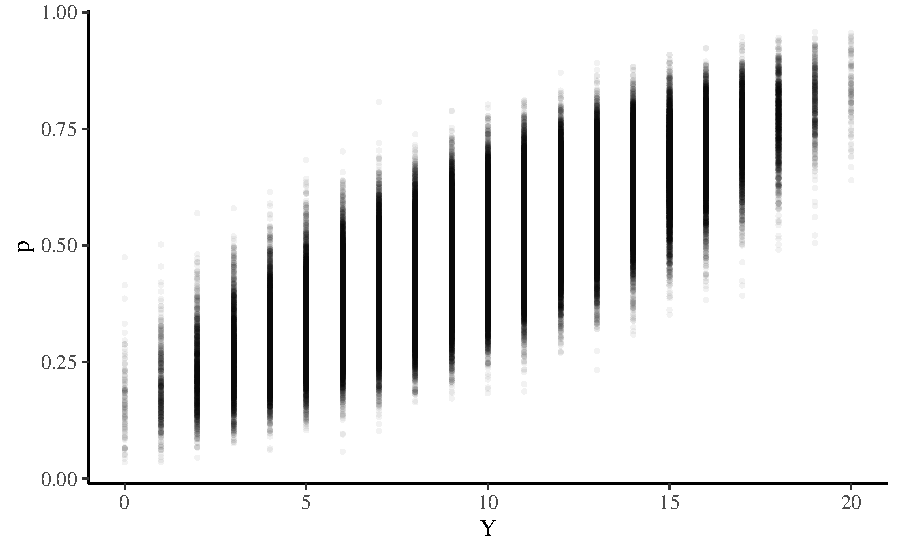
\includegraphics{ds4psy_files/figure-latex/unnamed-chunk-38-1} \end{center}

Mentre la media viene riprodotta accuratamente dal modello (come abbiamo visto sopra), ciò non è vero per il minimo dela distribuzione. L'origine di questa mancanza di adattamento è il fatto che la distribuzione delle misurazioni della velocità della luce è asimmetrica negativa. Dato che ci sono poche osservazioni nella coda negativa della distribuzione, solo per fare un esempio, utilizzeremo ora un secondo modello che ipotizza una distribuzione \(t\) di Student:

\begin{Shaded}
\begin{Highlighting}[]
\NormalTok{modelString }\OtherTok{\textless{}{-}} \StringTok{"}
\StringTok{data \{}
\StringTok{  int\textless{}lower=0\textgreater{} N;}
\StringTok{  vector[N] y;}
\StringTok{\}}
\StringTok{parameters \{}
\StringTok{  real mu;}
\StringTok{  real\textless{}lower=0\textgreater{} sigma;}
\StringTok{  real\textless{}lower=0\textgreater{} nu;}
\StringTok{\}}
\StringTok{model \{}
\StringTok{  mu \textasciitilde{} normal(25, 10);}
\StringTok{  sigma \textasciitilde{} cauchy(0, 10);}
\StringTok{  nu \textasciitilde{} cauchy(0, 10);}
\StringTok{  y \textasciitilde{} student\_t(nu, mu, sigma);}
\StringTok{\}}
\StringTok{generated quantities \{}
\StringTok{  vector[N] y\_rep;}
\StringTok{  for (n in 1:N) \{}
\StringTok{    y\_rep[n] = student\_t\_rng(nu, mu, sigma);}
\StringTok{  \}}
\StringTok{\}}
\StringTok{"}
\FunctionTok{writeLines}\NormalTok{(modelString, }\AttributeTok{con =} \StringTok{"code/newcomb2.stan"}\NormalTok{)}
\end{Highlighting}
\end{Shaded}

Adattiamo questo secondo modello ai dati.

\begin{Shaded}
\begin{Highlighting}[]
\NormalTok{file }\OtherTok{\textless{}{-}} \FunctionTok{file.path}\NormalTok{(}\StringTok{"code"}\NormalTok{, }\StringTok{"newcomb2.stan"}\NormalTok{)}
\NormalTok{mod }\OtherTok{\textless{}{-}} \FunctionTok{cmdstan\_model}\NormalTok{(file)}
\NormalTok{fit }\OtherTok{\textless{}{-}}\NormalTok{ mod}\SpecialCharTok{$}\FunctionTok{sample}\NormalTok{(}
  \AttributeTok{data =}\NormalTok{ data\_list,}
  \AttributeTok{iter\_sampling =}\NormalTok{ 4000L,}
  \AttributeTok{iter\_warmup =}\NormalTok{ 2000L,}
  \AttributeTok{seed =}\NormalTok{ SEED,}
  \AttributeTok{chains =}\NormalTok{ 4L,}
  \AttributeTok{cores =}\NormalTok{ 4L,}
  \AttributeTok{parallel\_chains =}\NormalTok{ 2L,}
  \AttributeTok{refresh =} \DecValTok{0}\NormalTok{,}
  \AttributeTok{thin =} \DecValTok{1}
\NormalTok{)}
\CommentTok{\#\textgreater{} Running MCMC with 4 parallel chains...}
\CommentTok{\#\textgreater{} }
\CommentTok{\#\textgreater{} Chain 1 finished in 0.3 seconds.}
\CommentTok{\#\textgreater{} Chain 2 finished in 0.3 seconds.}
\CommentTok{\#\textgreater{} Chain 3 finished in 0.3 seconds.}
\CommentTok{\#\textgreater{} Chain 4 finished in 0.3 seconds.}
\CommentTok{\#\textgreater{} }
\CommentTok{\#\textgreater{} All 4 chains finished successfully.}
\CommentTok{\#\textgreater{} Mean chain execution time: 0.3 seconds.}
\CommentTok{\#\textgreater{} Total execution time: 0.5 seconds.}
\end{Highlighting}
\end{Shaded}

Per questo secondo modello il confronto tra la funzione di densità empirica della \(y\) e quella di diversi campioni \(y^{rep}\) risulta adeguato:

\begin{Shaded}
\begin{Highlighting}[]
\NormalTok{stanfit }\OtherTok{\textless{}{-}}\NormalTok{ rstan}\SpecialCharTok{::}\FunctionTok{read\_stan\_csv}\NormalTok{(fit}\SpecialCharTok{$}\FunctionTok{output\_files}\NormalTok{())}
\NormalTok{y\_rep }\OtherTok{\textless{}{-}} \FunctionTok{as.matrix}\NormalTok{(stanfit, }\AttributeTok{pars =} \StringTok{"y\_rep"}\NormalTok{)}
\FunctionTok{ppc\_dens\_overlay}\NormalTok{(data\_list}\SpecialCharTok{$}\NormalTok{y, y\_rep[}\DecValTok{1}\SpecialCharTok{:}\DecValTok{50}\NormalTok{, ])}
\end{Highlighting}
\end{Shaded}

\begin{center}\includegraphics{ds4psy_files/figure-latex/unnamed-chunk-41-1} \end{center}

Inoltre, anche la statistica ``minimo della distribuzione'' viene ben predetta dal modello.

\begin{Shaded}
\begin{Highlighting}[]
\FunctionTok{ppc\_stat\_2d}\NormalTok{(data\_list}\SpecialCharTok{$}\NormalTok{y, y\_rep, }\AttributeTok{stat =} \FunctionTok{c}\NormalTok{(}\StringTok{"mean"}\NormalTok{, }\StringTok{"min"}\NormalTok{))}
\end{Highlighting}
\end{Shaded}

\begin{center}\includegraphics{ds4psy_files/figure-latex/unnamed-chunk-42-1} \end{center}

In conclusione, per le misurazioni della velocità della luce di Newcomb l'accuratezza predittiva del modello basato sulla distribuzione \(t\) di Student è chiaramente migliore di quella del modello normale.
\end{exercise}

\hypertarget{commenti-e-considerazioni-finali-1}{%
\section*{Commenti e considerazioni finali}\label{commenti-e-considerazioni-finali-1}}


Questo capitolo discute la predizione bayesiana e ne mostra un'applicazione nel caso dei controlli predittivi a posteriori. A questo proposito è necessario notare un punto importante: un buona corrispondenza tra \(y\) e \(y^{rep}\) costituisce una condizione necessaria ma non sufficiente per la validità del modello. Infatti, i PPC non sono in grado di garantire la generalizzabilità del modello a nuovi campioni di dati. D'altra parte, invece, se i PPC mostrano un cattivo adattamento del modello ai dati previsti futuri, questo ci dice chiaramente che il modello è specificato in manera errata.

  \bibliography{refs.bib,book.bib,packages.bib}

\printindex

\end{document}
